%!LW recipe=latexmk-xelatex
\documentclass[compress]{beamer}

\usetheme[block=fill]{metropolis}

\usepackage{graphicx} 
\usepackage{amsmath,amsfonts,amsthm,amssymb}
\usepackage{color}
\usepackage{xcolor,cancel}

\definecolor{mDarkBrown}{HTML}{604c38}
\definecolor{mDarkTeal}{HTML}{23373b}
\definecolor{mLightBrown}{HTML}{EB811B}
\definecolor{mMediumBrown}{HTML}{C87A2F}
\definecolor{mygreen}{HTML}{98C2B9}
\definecolor{myyellow}{HTML}{DFD79C}
\definecolor{myblue}{HTML}{8CA7CC}
\definecolor{kern}{HTML}{8CC2B7}


\usepackage{float}
\usepackage{framed}
\usepackage{epsfig}
\usepackage{graphicx}
\usepackage{subcaption}
\usepackage{ulem}
\usepackage{hhline}
\usepackage{multirow}
\usepackage{comment}   
\usepackage{bbm}
\usepackage{tikz}   
\def\Put(#1,#2)#3{\leavevmode\makebox(0,0){\put(#1,#2){#3}}}
\newcommand*\mystrut[1]{\vrule width0pt height0pt depth#1\relax}
\newcommand{\eqdef}{\mathbin{\stackrel{\rm def}{=}}}


\newcommand{\bs}[1]{\boldsymbol{#1}}
\newcommand{\bv}[1]{\mathbf{#1}}
\newcommand{\R}{\mathbb{R}}
\newcommand{\E}{\mathbb{E}}

\DeclareMathOperator{\vol}{vol}
\DeclareMathOperator*{\argmin}{arg\,min}
\DeclareMathOperator*{\argmax}{arg\,max}
\DeclareMathOperator{\nnz}{nnz}
\DeclareMathOperator{\Var}{Var}
\DeclareMathOperator{\diag}{diag}
\DeclareMathOperator{\sinc}{sinc}
\DeclareMathOperator{\sign}{sign}
\DeclareMathOperator{\dist}{dist}
\DeclareMathOperator{\mv}{mv}
\DeclareMathOperator{\sgn}{sgn}
\DeclareMathOperator{\step}{step}
\DeclareMathOperator{\gap}{gap}
\DeclareMathOperator{\poly}{poly}
\DeclareMathOperator{\tr}{tr}
\DeclareMathOperator{\orth}{orth}
\newcommand{\norm}[1]{\|#1\|}
\captionsetup[subfigure]{labelformat=empty}
\captionsetup[figure]{labelformat=empty}
\DeclareMathOperator*{\lmin}{\lambda_{min}}
\DeclareMathOperator*{\lmax}{\lambda_{max}}

\newcommand{\specialcell}[2][c]{%
  \begin{tabular}[#1]{@{}c@{}}#2\end{tabular}}
\newcommand{\specialcellleft}[2][c]{%
\begin{tabular}[#1]{@{}l@{}}#2\end{tabular}
}

\newtheorem{claim}[theorem]{Claim}

\usepackage{tabstackengine}
\stackMath


%----------------------------------------------------------------------------------------
%	TITLE PAGE
%----------------------------------------------------------------------------------------

\title{CS-GY 6763: Lecture 9 \\ Online and Stochastic Gradient Descent, Dimension Dependent Optimization}
\author{NYU Tandon School of Engineering, Prof. Christopher Musco}
\date{}

\begin{document}

\begin{frame}
	\titlepage 
\end{frame}

\metroset{titleformat=smallcaps}

\begin{frame}
	\frametitle{standard optimization setting}
	Given a function $f$ to minimize, assume we have:
	\begin{itemize}
		\item \textbf{Function oracle}: Evaluate $f(\bv{x})$ for any $\bv{x}$. 
		\item \textbf{Gradient oracle}: Evaluate $\nabla f(\bv{x})$ for any $\bv{x}$.
	\end{itemize}
	\textbf{Goal:} Minimize the number of oracle calls to find $\tilde{\bv{x}}$ such that $f(\tilde{\bv{x}}) \leq \min_{\bv{x}}f(\bv{x}) + \epsilon$. 

	\begin{center}
	In machine learning applications,  $f(\bv{x})$ is typically  a loss function for a fixed training dataset. 
	\end{center}
\end{frame}

\begin{frame}[t]
	\frametitle{online and stochastic gradient descent}
	\textbf{First part of class:}
	\begin{itemize}
		\item Basics of an alternative setting: \emph{Online Learning + Optimization}. 
		\item Introduction to \emph{Regret Analysis}.
		\item Application to analyzing \emph{Stochastic Gradient Descent.}
	\end{itemize}
	
\end{frame}


\begin{frame}
	\frametitle{online learning}
	\begin{center}
		\textbf{Many machine learning problems are solved in an \emph{online} setting with constantly changing data.}
	\end{center}
	\begin{itemize}
		\item Spam filters are incrementally updated and adapt as they see more examples of spam over time. 
		\item Text recommendation engines (e.g. Github Copilot) need to be kept up-to-date as software libraries/APIs change.
		\item Content recommendation systems adapt to user behavior and clicks (which may not be a good thing...)
	\end{itemize}
\end{frame}

\begin{frame}
	\frametitle{example}
	\begin{center}
		\textbf{Machine learning  based email spam filtering.}
	\end{center}
	\begin{center}
		
\includegraphics[width=.5\textwidth]{covid_spam.png}
	\end{center}
	Markers for spam change overtime, so model might change.
\end{frame}

\begin{frame}
	\frametitle{example}
	\begin{center}
	\textbf{Plant identification via iNaturalist app.}
		
	(California Academy of Science + National Geographic)
	\end{center}
\begin{columns}
	\begin{column}{.5\textwidth}
		\centering
		
\includegraphics[width=.5\textwidth]{inaturalist.png}
	\end{column}
	\begin{column}{.5\textwidth}
		\begin{itemize}
			\item When the app fails, image is classified via crowdsourcing (backed by huge network of amateurs and experts).
		
			\item Single model that is updated constantly, not retrained in batches.
		\end{itemize}
	\end{column}
\end{columns}
\end{frame}

\begin{frame}
	\frametitle{online learning framework}
	Choose some model $M_\bv{x}$ parameterized by parameters $\bv{x}$ and some loss function $\ell$. 
	At time steps $1,\ldots, T$, receive data vectors $\bv{a}^{(1)}, \ldots, \bv{a}^{(T)}$. 
	\begin{itemize}
		\item At each time step, we pick (``play'') a parameter vector $\bv{x}^{(i)}$.
		\item Make prediction $\tilde{y}^{(i)} = M_{\bv{x}^{(i)}}(\bv{a}_i)$.
		\item Then told true value or label $y^{(i)}$. Possibly use this information to choose a new $\bv{x}^{(i+1)}$.
		\item Goal is to minimize cumulative loss:
		\begin{align*}
			L = \sum_{i=1}^n \ell(\bv{x}^{(i)}, \bv{a}^{(i)}, y^{(i)})
		\end{align*} 
	\end{itemize}
	For example, for a regression problem we might use the $\ell_2$ loss:
	\begin{align*}
		\ell(\bv{x}^{(i)}, \bv{a}^{(i)}, y^{(i)}) = \left|\langle\bv{x}^{(i)},\bv{a}^{(i)}\rangle - y^{(i)}\right|^2. 
	\end{align*}
For classification, we could use logistic/cross-entropy loss. 
\end{frame}

\begin{frame}
	\frametitle{online optimization}
	\textbf{Abstraction as optimization problem:} Instead of a single objective function $f$, we have a single (initially unknown) function $f_1, \ldots, f_T: \R^d \rightarrow \R$ for each time step. 
	\begin{itemize}
		\item For time step $i\in 1,\ldots, T$, select vector $\bv{x}^{(i)}$.
		\item Observe $f_i$ and pay cost $f_i(\bv{x}^{(i)})$
		\item Goal is to minimize $\sum_{i=1}^T f_i(\bv{x}^{(i)})$. 
	\end{itemize}

	\begin{center}
		We make \emph{no assumptions} that $f_1, \ldots, f_T$ are related to each other at all!
	\end{center}
\end{frame}

\begin{frame}[t]
	\frametitle{regret bound}
	In offline optimization, we wanted to find $\hat{\bv{x}}$ satisfying $f(\hat{\bv{x}}) \leq \min_{\bv{x}} f(\bv{x})$. Ask for a similar thing here. 
	
	\textbf{Objective:} Choose $\bv{x}^{(1)}, \ldots, \bv{x}^{(T)}$ so that: 
	\begin{align*}
		\sum_{i=1}^T f_i(\bv{x}^{(i)}) \leq \left[\min_\bv{x} \sum_{i=1}^T f_i(\bv{x})\right] + \epsilon.
	\end{align*}
	Here $\alert{\epsilon}$ is called the \alert{\textbf{regret}} of our solution sequence $\bv{x}^{(1)}, \ldots, \bv{x}^{(T)}$. 		Regret compares to the best \emph{fixed solution} in hindsight.

	
	We typically $\epsilon$ to be growing \emph{sublinearly} in $T$. 
\end{frame}

\begin{frame}[t]
	\frametitle{regret bound}
	\begin{center}
		Regret compares to the best \emph{fixed} solution in hindsight.
	\end{center}
	\begin{align*}
		\sum_{i=1}^T f_i(\bv{x}^{(i)}) \leq \left[\min_\bv{x} \sum_{i=1}^T f_i(\bv{x})\right] + \epsilon.
	\end{align*}
	It's very possible that $\sum_{i=1}^T f_i(\bv{x}^{(i)}) < \left[\min_\bv{x} \sum_{i=1}^T f_i(\bv{x})\right]$. Could we hope for something stronger?
	
	\textbf{Exercise:} Argue that the following is impossible to achieve:
	\begin{align*}
		\sum_{i=1}^T f_i(\bv{x}^{(i)}) \leq \left[\sum_{i=1}^T \min_\bv{x} f_i(\bv{x})\right] + \epsilon.
	\end{align*}
\end{frame}

\begin{frame}[t]
	\frametitle{hard example for online optimization}
	\textbf{Convex functions:}
	\begin{align*}
		f_1(x) &= |x - h_1|\\
		 &\vdots\\
		 f_n(x) &= |x - h_T|
	\end{align*}
where $h_1, \ldots, h_T$ are i.i.d. uniform $\{0,1\}$.
\end{frame}

\begin{frame}[t]
	\frametitle{regret bounds}
	\begin{align*}
		\sum_{i=1}^T f_i(\bv{x}^{(i)}) \leq \left[\min_\bv{x} \sum_{i=1}^T f_i(\bv{x})\right] + \epsilon.
	\end{align*}
	
	\textbf{Beautiful balance:}
	\begin{itemize}
		\item Either $f_1, \ldots, f_T$ are similar or changing slowly, so we can learn predict $f_i$ from earlier functions.
		\item Or $f_1, \ldots, f_T$  are very different, in which case $\min_\bv{x} \sum_{i=1}^T f_i(\bv{x})$ is large, so regret bound is easy to achieve. 
		\item Or we live somewhere in the middle.
	\end{itemize} 
\end{frame}

\begin{frame}[t]
	\frametitle{follow-the-leader}
		\textbf{Follow-the-leader algorithm:}
	\begin{itemize}
		\item Choose $\bv{x}^{(0)}$.
		\item For $i = 1,\ldots, T$:
		\begin{itemize}
			\item Let $\bv{x}^{(i)} = \argmin_{\bv{x}} \sum_{j=1}^{i-1} f_j(\bv{x})$.
			\item Play $\bv{x}^{(i)}$.
			\item Observe $f_{i}$ and incur cost $f_{i}(\bv{x}^{(i)})$. 
		\end{itemize}
	\end{itemize}
Simple and intuitive, but there are \emph{two} issues with this approach. One is computational, one is related to the accuracy.
	
\end{frame}

\begin{frame}[t]
	\frametitle{follow-the-leader}
	\textbf{Hard case:}
\begin{center}
	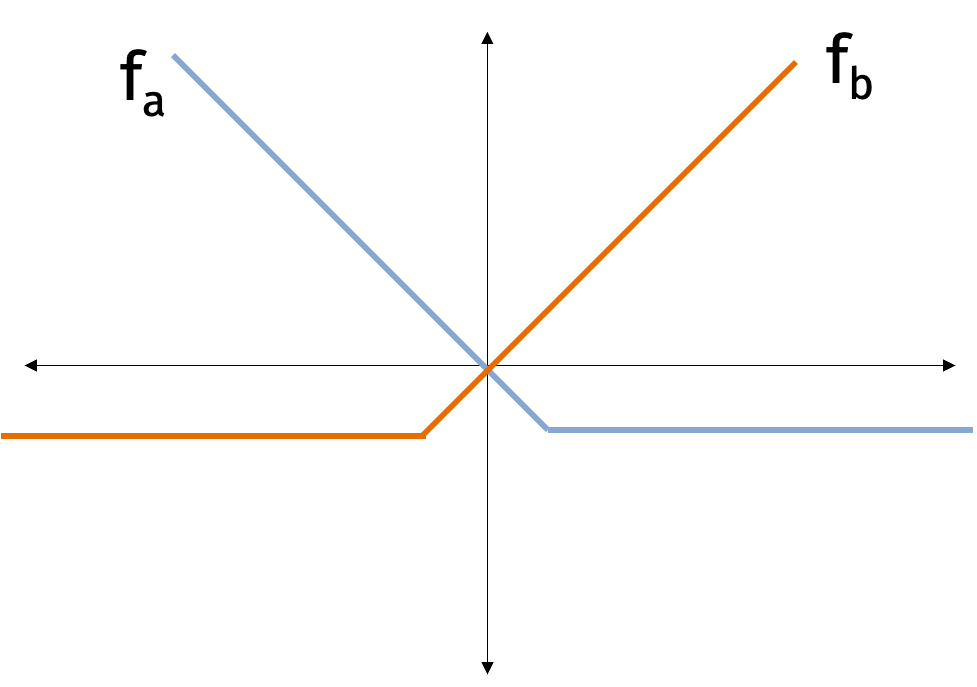
\includegraphics[width=.7\textwidth]{hard_case_ftl.png}
	\end{center}
\end{frame}


\begin{frame}[t]
	\frametitle{online gradient descent}
	\textbf{Online Gradient descent:}
\begin{itemize}
	\item Choose $\bv{x}^{(1)}$ and $\eta = \frac{R}{G\sqrt{T}}$. 
	\item For $i = 1,\ldots, T$:
	\begin{itemize}
		\item Play $\bv{x}^{(i)}$.
		\item Observe $f_{i}$ and incur cost $f_{i}(\bv{x}^{(i)})$. 
		\item $\bv{x}^{(i+1)} = \bv{x}^{(i)} - \eta \nabla f_i(\bv{x}^{(i)})$
	\end{itemize}
\end{itemize}
If $f_1, \ldots, f_T = f$ are all the same, this is the same as regular gradient descent. We update parameters using the gradient $\nabla f$ at each step. 
\end{frame}

\begin{frame}[t]
	\frametitle{online gradient descent (ogd)}
	$\bv{x}^{*} = \argmin_\bv{x}\sum_{i=1}^T f_i(\bv{x})$ (the offline optimum)
	
	\textbf{Assume:}
	\begin{itemize}
		\item $f_1, \ldots, f_T$ are all convex.
		\item Each is $G$-Lipschitz: for all $\bv{x}$, $i$, $\|\nabla f_i(\bv{x})\|_2 \leq \alert{G}$.
		\item Starting radius: $\|\bv{x}^{*} - \bv{x}^{(1)}\|_2 \leq \alert{R}$.
	\end{itemize}
	
	\textbf{Online Gradient descent:}
	\begin{itemize}
	\item Choose $\bv{x}^{(1)}$ and $\eta = \frac{R}{G\sqrt{T}}$. 
	\item For $i = 1,\ldots, T$:
	\begin{itemize}
		\item Play $\bv{x}^{(i)}$.
		\item Observe $f_{i}$ and incur cost $f_{i}(\bv{x}^{(i)})$. 
		\item $\bv{x}^{(i+1)} = \bv{x}^{(i)} - \eta \nabla f_i(\bv{x}^{(i)})$
	\end{itemize}
\end{itemize}
\end{frame}

\begin{frame}[t]
	\frametitle{online gradient descent analysis} 
Let $\bv{x}^{*} = \argmin_\bv{x}\sum_{i=1}^T f_i(\bv{x})$ (the offline optimum)
	\begin{theorem}[OGD Regret Bound]
		After $T$ steps, $\epsilon = \left[\sum_{i=1}^T f_i(\bv{x}^{(i)})\right] - \left[\sum_{i=1}^T f_i(\bv{x}^*)\right] \leq RG\sqrt{T}$.
	\end{theorem}
	Average regret overtime is bounded by $\frac{\epsilon}{T} \leq \frac{RG}{\sqrt{T}}$.
	
	Goes $\rightarrow 0$ as $T\rightarrow \infty$. 
	
	\begin{center}
		All this with no assumptions on how $f_1, \ldots, f_T$ relate to each other! They could have even been chosen \alert{\textbf{adversarially}} -- e.g. with $f_i$ depending on our choice of $\bv{x}_i$ and all previous choices. 
	\end{center}
\end{frame}

\begin{frame}[t]
	\frametitle{online gradient descent analysis}
	\begin{theorem}[OGD Regret Bound]
		After $T$ steps, $\epsilon = \left[\sum_{i=1}^T f_i(\bv{x}^{(i)})\right] - \left[\sum_{i=1}^T f_i(\bv{x}^*)\right] \leq RG\sqrt{T}$.
	\end{theorem}
	\textbf{Claim 1:} For all $i = 1, \ldots, T$, 
	\begin{align*}
		f_i(\bv{x}^{(i)}) - f_i(\bv{x}^*) \leq \frac{\|\bv{x}^{(i)} - \bv{x}^*\|_2^2 - \|\bv{x}^{(i+1)} - \bv{x}^*\|_2^2}{2\eta} + \frac{\eta G^2}{2}
	\end{align*}
(Same proof for standard GD. Only uses convexity of $f_i$.)

\end{frame}

\begin{frame}[t]
	\frametitle{online gradient descent analysis}
	\begin{theorem}[OGD Regret Bound]
		After $T$ steps, $\epsilon = \left[\sum_{i=1}^T f_i(\bv{x}^{(i)})\right] - \left[\sum_{i=1}^T f_i(\bv{x}^*)\right] \leq RG\sqrt{T}$.
	\end{theorem}
	\textbf{Claim 1:} For all $i = 1, \ldots, T$, 
	\begin{align*}
		f_i(\bv{x}^{(i)}) - f_i(\bv{x}^*) \leq \frac{\|\bv{x}^{(i)} - \bv{x}^*\|_2^2 - \|\bv{x}^{(i+1)} - \bv{x}^*\|_2^2}{2\eta} + \frac{\eta G^2}{2}
	\end{align*}
	\textbf{Telescoping Sum:} 
	\begin{align*}
		\sum_{i=1}^{T}\left[f_i(\bv{x}^{(i)}) - f_i(\bv{x}^*)\right] &\leq \frac{\|\bv{x}^{(1)}-\bv{x}^*\|_2^2 -\|\bv{x}^{(T)}-\bv{x}^*\|_2^2}{2\eta} + \frac{T\eta G^2}{2} \\ &\leq  \frac{R^2}{2\eta} + \frac{T\eta G^2}{2}
	\end{align*}
	
	
\end{frame}

\begin{frame}
	\frametitle{stochastic gradient descent (sgd)}
	Efficient \emph{offline} optimization method for functions $f$ with \emph{finite sum structure}:
	\begin{align*}
		f(\bv{x}) = \sum_{i=1}^n f_i(\bv{x}).
	\end{align*}
	
	
	Goal is to find $\hat{\bv{x}}$ such that $f(\hat{\bv{x}}) \leq f(\bv{x}^*) + \epsilon$. 
	
	\begin{itemize}
		\item The most widely use optimization algorithm in modern machine learning. 
		\item Easily analyzed as a special case of {online} gradient descent! 
	\end{itemize}
\end{frame}

\begin{frame}[t]
	\frametitle{stochastic gradient descent}
	Recall the machine learning setup. In empirical risk minimization, we can typically write:
	\begin{align*}
		f(\bv{x}) = \sum_{i=1}^n f_i(\bv{x})
	\end{align*}
	where $f_i$ is the loss function for a particular data example $(\bv{a}^{(i)},y^{(i)} )$.
	\vspace{1em}
	
	\textbf{Example: least squares linear regression.}
	\begin{align*}
		f(\bv{x}) = \sum_{i=1}^n (\bv{x}^T\bv{a}^{(i)} - y^{(i)})^2
	\end{align*}
Note that by linearity, $\nabla f(\bv{x}) = \sum_{i=1}^n \nabla f_i(\bv{x})$. 
\end{frame}

\begin{frame}
	\frametitle{stochastic gradient descent}
	{\textbf{Main idea:} Use random approximate gradient in place of actual gradient.}
	
	Pick \emph{random} $j \in 1, \ldots, n$ and update $\bv{x}$  using $\nabla f_j(\bv{x})$. 
	\begin{align*}
		\E\left[\nabla f_j(\bv{x})\right] = \frac{1}{n}\nabla f(\bv{x}).
	\end{align*}

\vspace{2em}
	$n \nabla f_j(\bv{x})$ is an unbiased estimate for the true gradient $\nabla f(\bv{x})$, but can typically be computed in a $1/n$ fraction of the time!
	

	
	\begin{center}
		\alert{\textbf{Trade slower convergence for cheaper iterations.}}
	\end{center}
\end{frame}


\begin{frame}[t]
	\frametitle{stochastic gradient descent}
   {Stochastic first-order oracle} for $f(\bv{x}) = \sum_{i=1}^n f_i(\bv{x})$. 
	\begin{itemize}
		\item \textcolor{lightgray}{ \textbf{Function Query:} For any chosen $j, \bv{x}$, return $f_j(\bv{x})$}
		\item \textbf{Gradient Query:} For any chosen $j, \bv{x}$, return $\nabla f_j(\bv{x})$
	\end{itemize}
%	Computing $f(\bv{x})$ would take $n$ separate function queries. 

	\textbf{Stochastic Gradient descent:}
	\begin{itemize}
		\item Choose starting vector $\bv{x}^{(1)}$, step size $\eta$
		\item For $i = 1,\ldots, T$:
		\begin{itemize}
			\item Pick random $j_i$ uniformly at random from $1, \ldots, n$.
			\item $\bv{x}^{(i+1)} = \bv{x}^{(i)} - \eta \nabla f_{j_i}(\bv{x}^{(i)})$
		\end{itemize}
		\item Return $\hat{\bv{x}} = \frac{1}{T}\sum_{i=1}^T \bv{x}^{(i)}$
	\end{itemize}
\end{frame}

\begin{frame}[t]
	\frametitle{visualizing sgd}
	\begin{center}
		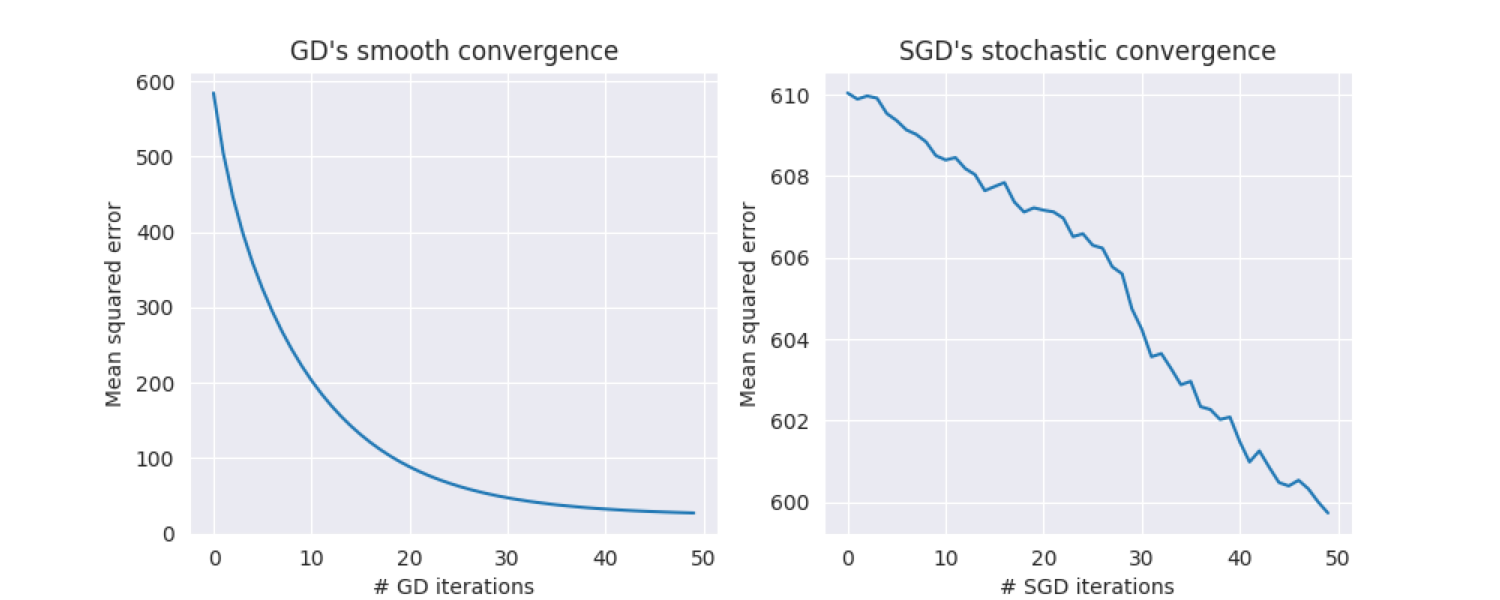
\includegraphics[height=.45\textheight]{gd_convergence.png}
		
		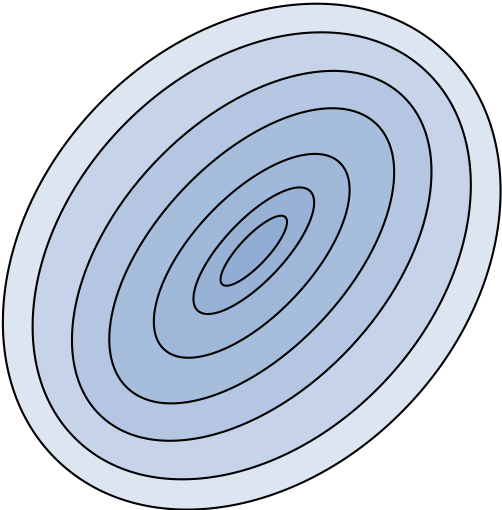
\includegraphics[height=.4\textheight]{gd_paths_raw.png}
	\end{center}	
\end{frame}


\begin{frame}[t]
	\frametitle{stochastic gradient descent}
	\small
		\vspace{-.5em}
	\textbf{Assume:}
	\vspace{-1em}
	\begin{itemize}
		\item {Finite sum structure:} $f(\bv{x}) = \sum_{i=1}^n f_i(\bv{x})$, with $f_1, \ldots, f_n$ all convex.
		\item {Lipschitz functions}: for all $\bv{x}$, $j$, $\|\nabla f_j(\bv{x})\|_2 \leq \alert{\frac{G'}{n}}$.
		\begin{itemize}
			\item What does this imply about Lipschitz constant of $f$?
		\end{itemize}
		\item Starting radius: $\|\bv{x}^{*} - \bv{x}^{(1)}\|_2 \leq \alert{R}$.
	\end{itemize}
	
	\vspace{-.5em}
	\textbf{Stochastic Gradient descent:}
	\vspace{-1em}
	\begin{itemize}
		\item Choose $\bv{x}^{(1)}$, steps $T$, step size $\eta = \frac{R}{G'\sqrt{T}}$.
		\item For $i = 1,\ldots, T$:
		\begin{itemize}
			\item Pick random $j_i \in 1, \ldots, n$.
			\item $\bv{x}^{(i+1)} = \bv{x}^{(i)} - \eta \nabla f_{j_i}(\bv{x}^{(i)})$
		\end{itemize}
		\item Return $\hat{\bv{x}} = \frac{1}{T}\sum_{i=1}^T \bv{x}^{(i)}$
	\end{itemize}
\alert{	\textbf{Approach: View as online gradient descent run on function sequence $f_{j_1}, \ldots, f_{j_T}$.} } 

Only use the fact that step equals gradient in expectation.
\end{frame}


\begin{frame}[t]
	\frametitle{jensen's inequality}
	For a convex function $f$ and points $\bv{x}^{(1)}, \ldots, \bv{x}^{(t)}$
	\begin{align*}
	f\left(\frac{1}{t}\cdot \bv{x}^{(1)} + \ldots + \frac{1}{t}\cdot \bv{x}^{(t)} \right) \leq \frac{1}{t}\cdot f(\bv{x}^{(1)}) + \ldots +\frac{1}{t} \cdot f(\bv{x}^{(t)} )
	\end{align*}
	
\end{frame}

\begin{frame}[t]
	\frametitle{stochastic gradient descent analysis}
	\begin{claim}[SGD Convergence]
		After $T = \frac{R^2G'^2}{\epsilon^2}$ iterations:
		\begin{align*}
			\E\left[f(\hat{\bv{x}}) - f(\bv{x}^*)\right] \leq \epsilon.
		\end{align*}

	\end{claim}
	\textbf{Claim 1:} 
	\begin{align*}
		f(\hat{\bv{x}}) - f(\bv{x}^*) \leq \frac{1}{T}\sum_{i=1}^T\left[f(\bv{x}^{(i)}) -f(\bv{x}^*)\right]
	\end{align*}
\textbf{Prove using Jensen's Inequality:}
\end{frame}

\begin{frame}[t]
	\frametitle{stochastic gradient descent analysis}
	\small
	\begin{claim}[SGD Convergence]
		After $T = \frac{R^2G'^2}{\epsilon^2}$ iterations:
		\vspace{-1em}
		\begin{align*}
			\E\left[f(\hat{\bv{x}}) - f(\bv{x}^*)\right] \leq \epsilon.
		\end{align*}
	
		\vspace{-1em}
	\end{claim}\vspace{-2em}
	\begin{align*}
		\E[f(\hat{\bv{x}}) - f(\bv{x}^*)] &\leq \frac{1}{T}\sum_{i=1}^T\E\left[f(\bv{x}^{(i)}) -f(\bv{x}^*)\right]
		\\
		&=\frac{1}{T}\sum_{i=1}^Tn\E\left[f_{j_i}(\bv{x}^{(i)}) -f_{j_i}(\bv{x}^*)\right]\\
		&=\frac{n}{T}\cdot \E \left[\sum_{i=1}^Tf_{j_i}(\bv{x}^{(i)}) -f_{j_i}(\bv{x}^*)\right]
	\end{align*}
\end{frame}

\begin{frame}[t]
	\frametitle{stochastic gradient descent analysis}
	\small
	\begin{claim}[SGD Convergence]
		After $T = \frac{R^2G'^2}{\epsilon^2}$ iterations:
		\vspace{-1em}
		\begin{align*}
			\E\left[f(\hat{\bv{x}}) - f(\bv{x}^*)\right] \leq \epsilon.
		\end{align*}
		
		\vspace{-1em}
	\end{claim}\vspace{-2em}
	\begin{align*}
		\E[f(\hat{\bv{x}}) - f(\bv{x}^*)] &\leq \frac{1}{T}\sum_{i=1}^T\E\left[f(\bv{x}^{(i)}) -f(\bv{x}^*)\right]
		\\
		&=\frac{1}{T}\sum_{i=1}^Tn\E\left[f_{j_i}(\bv{x}^{(i)}) -f_{j_i}(\bv{x}^*)\right]\\
		&\leq \frac{n}{T}\cdot \E\left[\sum_{i=1}^T f_{j_i}(\bv{x}^{(i)}) -f_{j_i}(\bv{x}^{offline})\right], 
	\end{align*}
where $\bv{x}^{offline} = \argmin_{\bv{x}}\sum_{i=1}^{T} f_{j_i}(\bv{x})$.
\end{frame}

\begin{frame}[t]
	\frametitle{stochastic gradient descent analysis}
	\small
	\begin{claim}[SGD Convergence]
		After $T = \frac{R^2G'^2}{\epsilon^2}$ iterations:
		\vspace{-1em}
		\begin{align*}
			\E\left[f(\hat{\bv{x}}) - f(\bv{x}^*)\right] \leq \epsilon.
		\end{align*}
		
		\vspace{-1em}
	\end{claim}\vspace{-2em}
	\begin{align*}
		\E[f(\hat{\bv{x}}) - f(\bv{x}^*)] &\leq \frac{1}{T}\sum_{i=1}^T\E\left[f(\bv{x}^{(i)}) -f(\bv{x}^*)\right]
		\\
		&=\frac{1}{T}\sum_{i=1}^Tn\E\left[f_{j_i}(\bv{x}^{(i)}) -f_{j_i}(\bv{x}^*)\right]\\
		&\leq\frac{n}{T}\E\left[\sum_{i=1}^T f_{j_i}(\bv{x}^{(i)}) -f_{j_i}(\bv{x}^{offline})\right]\\
		& \leq \frac{n}{T} \cdot\left(R\cdot\frac{G'}{n}\cdot \sqrt{T}\right) \text{\hspace{2em} (by OGD guarantee.)}
	\end{align*}
\end{frame}


\begin{frame}[t]
	\frametitle{stochastic vs. full batch gradient descent}
	Number of iterations for error $\epsilon$:
	\begin{itemize}
		\item \textbf{Gradient Descent}: $T = \frac{R^2 G^2}{\epsilon^2}$. 
		\item \textbf{Stochastic Gradient Descent}: $T = \frac{R^2 G'^2}{\epsilon^2}$. 
	\end{itemize}
	
	\textbf{Always have $G \leq G'$:}
	\begin{align*}
		\max_{\bv{x}} \|\nabla f(\bv{x})\|_2 &\leq\max_{\bv{x}}\left( \|\nabla f_1(\bv{x})\|_2 + \ldots + \|\nabla f_n(\bv{x})\|_2\right) \\
		&\leq \max_{\bv{x}}\left( \|\nabla f_1(\bv{x})\|_2\right)+ \ldots + \max_{\bv{x}}\left( \|\nabla f_n(\bv{x})\|_2\right) \\
		&\leq n\cdot\frac{G'}{n} = G'.
	\end{align*}
So GD converges strictly faster than $SGD$. 
	
	\textbf{But for a fair comparison:}
	\begin{itemize}
		\item SGD cost = $(\# \text{ of iterations})\cdot O(1)$
		\item GD cost = $(\# \text{ of iterations})\cdot O(n)$
	\end{itemize}
\end{frame}

\begin{frame}[t]
	\frametitle{stochastic vs. full batch gradient descent}
	We always have $G \leq G'$. When it is \emph{much smaller} then GD will perform better. When it is closer to this upper bound, SGD will perform better. 
	
	\begin{center}
	What is an extreme case where $G = G'$? 
	\end{center}
\end{frame}

\begin{frame}[t]
	\frametitle{stochastic vs. full batch gradient descent}
	What if each gradient $\nabla f_i(\bv{x})$ looks like random vectors in $\R^d$? E.g. with $\mathcal{N}(0,1)$ entries? 
	
	\begin{align*}
		\E \left[\|\nabla f_i(\bv{x})\|_2^2\right] = \hspace{17em}
	\end{align*}
	\begin{align*}
		\E \left[\|\nabla f(\bv{x})\|_2^2\right] = \E \left[\|\sum_{i=1}^n\nabla f_i(\bv{x})\|_2^2\right] = \hspace{8em}
	\end{align*}

\vspace{5em}

\end{frame}

\begin{frame}
\frametitle{stochastic vs. full batch gradient descent}
\begin{center}
	\textbf{Takeaway:} SGD performs better when there is more structure or repetition in the data set. 
	
	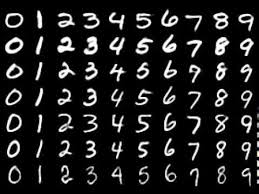
\includegraphics[height=.4\textheight]{mnist.jpeg}\hspace{2em}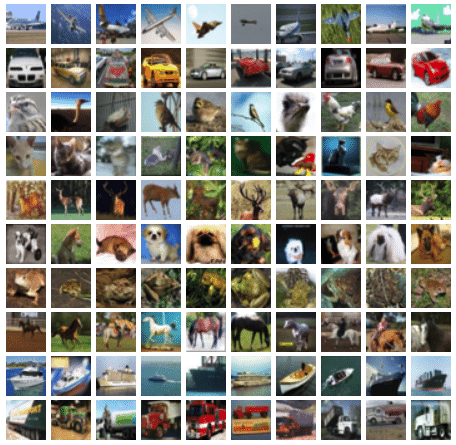
\includegraphics[height=.4\textheight]{cifar10.png}
\end{center}

\end{frame}

\begin{frame}[standout]
	\begin{center}
		\large preconditioning
	\end{center}
\end{frame}

\begin{frame}
	\frametitle{preconditioning}
	\textbf{Main idea:}
	Instead of minimizing $f(\bv{x})$, find another function $g(\bv{x})$ with the same minimum but which is better suited for first order optimization (e.g., has a smaller conditioner number).
	
	\vspace{2em}
	\textbf{Claim:} Let $h(\bv{x}): \R^d \rightarrow \R^d$ be an \emph{invertible function}. Let $g(\bv{x}) = f(h(\bv{x}))$. Then
	\begin{align*}
		\alert{\min_{\bv{x}} f(\bv{x})} &\alert{= \min_{\bv{x}} g(\bv{x})} & &\text{and} & \alert{\argmin_{\bv{x}} f(\bv{x})} &\alert{= h\left(\argmin_{\bv{x}} g(\bv{x})\right)}.
	\end{align*}
\end{frame}

\begin{frame}[t]
	\frametitle{preconditioning}
	\textbf{First Requirement:} We need $g(\bv{x})$ to still be convex.
	
	\textbf{Claim:} Let $\bv{P}$ be an invertible $d\times d$ matrix and let $g(\bv{x}) = f(\bv{P}\bv{x})$. 
	\begin{center} 
		\alert{$g(\bv{x})$ is always convex.}
	\end{center}

\vspace{2em}
	For this choice of preconditioner, if $\tilde{\bv{x}} \approx \argmin g(\bv{x})$, we would want to return $\textbf{P}\tilde{\bv{x}}$ as a near minimizer of $f$.
\end{frame}

\begin{frame}[t]
	\frametitle{preconditioning}
	\textbf{Additional Goals:} 
	\begin{itemize}
		\item $g(\bv{x})$ should be better conditioned (more smooth, more strongly convex, etc.) than $f$. 
		\item $\bv{P}$ needs to be easy to compute and we need to be able to apply $\bv{P}\bv{x}$ efficiently.
	\end{itemize}

	\textbf{Common choice:} Diagonal preconditioner. 
	\begin{itemize}
		\item Choose $\bv{P}$ to be a diagonal matrix $\bv{D}$. 
		\item For $f(\bv{x}) = \|\bv{A}\bv{x} - \bv{b}\|_2^2$, common choice is $\bv{D} = \diag(\bv{A}^T\bv{A})^{-1}$, which is known as the \textbf{Jacobi preconditioner}.
	\end{itemize}
	Often works very well in practice!
\end{frame}

\begin{frame}
	\frametitle{diagonal preconditioner}
	\begin{center}
		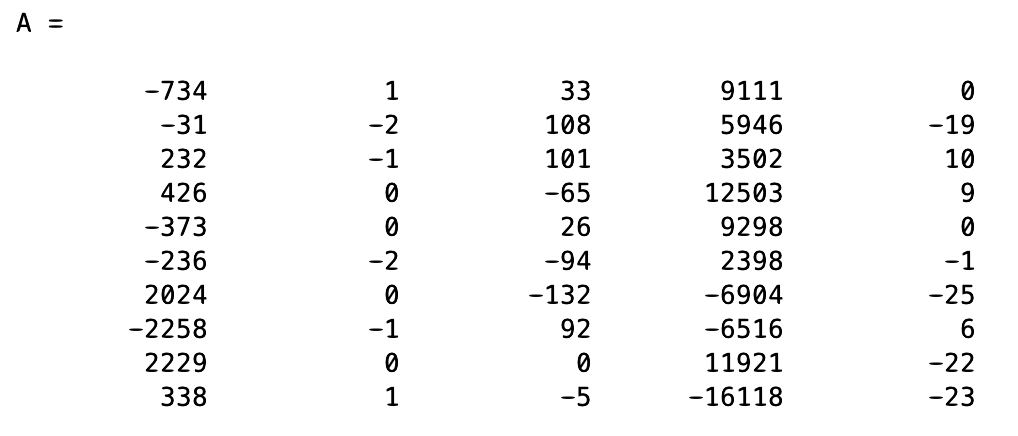
\includegraphics[width=.7\textwidth]{poorly_cond_a.png}
	\end{center}
	\vspace{2em}
	
	\begin{columns}[t]
		\begin{column}{0.3\textwidth}
			\vspace{-6.4em}
			
			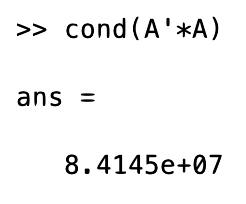
\includegraphics[width=.8\textwidth]{cond1.png}
		\end{column}
		\begin{column}{0.7\textwidth}
			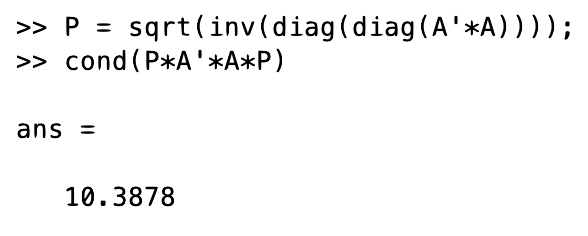
\includegraphics[width=.8\textwidth]{cond2.png}
		\end{column}
	\end{columns}
\end{frame}

%\begin{frame}
%	\frametitle{diagonal preconditioner}
%	\begin{center}
%		\alert{Can you think of an example $\bv{A}$ where Jacobi preconditioning doesn't decrease a large $\kappa$?}
%	\end{center}
%	\vspace{3em}
%		\begin{center}
%		\alert{Can Jacobi preconditioning \emph{increase} $\kappa$?}
%	\end{center}
%\end{frame}


\begin{frame}
	\frametitle{adaptive stepsizes}
	\textbf{Another view}: If $g(\bv{x}) = f(\bv{P}\bv{x})$ then $\nabla g(\bv{x}) = \bv{P}^T\nabla f(\bv{P}\bv{x})$.
	
	$\nabla g(\bv{x})  = \bv{P}\nabla f(\bv{P}\bv{x})$ when $\bv{P}$ is symmetric. 
	
	\vspace{1em}
	\textbf{Gradient descent on $g$:}
	\begin{itemize}
		\item For $t = 1,\ldots, T$,
		\begin{itemize}
			\item $\bv{x}^{(t+1)} = \bv{x}^{(t)} - \eta\bv{P}\left[\nabla f(\bv{P}\bv{x}^{(t)})\right]$
		\end{itemize}
	\end{itemize}
	
	\vspace{1em}
	\textbf{Gradient descent on $g$:}
	\begin{itemize}
		\item For $t = 1,\ldots, T$,
		\begin{itemize}
			\item $\bv{y}^{(t+1)} = \bv{y}^{(t)} - \eta\bv{P}^2\left[\nabla f(\bv{y}^{(t)})\right]$
		\end{itemize}
	\end{itemize}
	\begin{center}
		\alert{When $\bv{P}$ is diagonal, this is just gradient descent with a \emph{different step size for each parameter}!}
	\end{center}
\end{frame}

\begin{frame}
	\frametitle{adaptive stepsizes}
	\textbf{Algorithms based on this idea:}
	\begin{itemize}
		\item AdaGrad
		\item RMSprop
		\item Adam optimizer
	\end{itemize}
	\begin{center}
		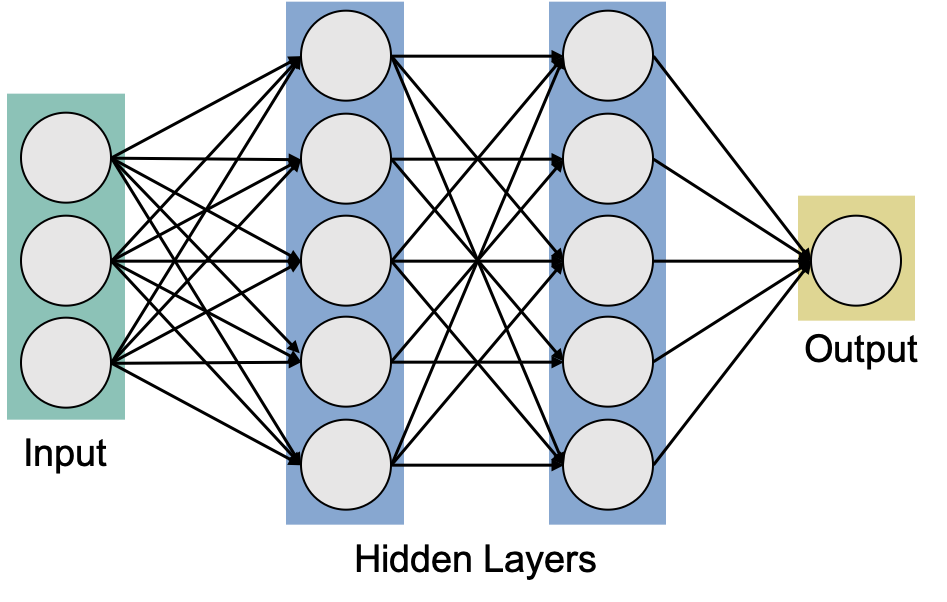
\includegraphics[width=.5\textwidth]{neuralNetwork.png}
		
		\alert{(Pretty much all of the most widely used optimization methods for training neural networks.)}
	\end{center}
\end{frame}

\begin{frame}[standout]
	\begin{center}
		\large break
	\end{center}
\end{frame}

% \begin{frame}
% 	\frametitle{stochastic methods}
% 	\textbf{Main idea:} Trade slower convergence (more iterations) for cheaper iterations. 
% 	\vspace{2em}
	
% 	\textbf{Stochastic Gradient Descent:}
% 	When $f(\bv{x}) = \sum_{i=1}^n f_i(\bv{x})$, approximate $\nabla f(\bv{x})$ with $\nabla f_i(\bv{x})$ for randomly chosen $i$. 
% \end{frame}

% \begin{frame}
% 	\frametitle{stochastic methods}
% 	\textbf{Main idea:} Trade slower convergence (more iterations) for cheaper iterations. 
% 	\vspace{2em}
	
% 	\textbf{Stochastic \alert{Coordinate Descent}:}
% 	Only compute a \emph{single random entry} of $\nabla f(\bv{x})$ on each iteration:
% 	\begin{align*}
% 		\nabla f(\bv{x}) &= 
% 		\begin{bmatrix}
% 			\frac{\partial f}{\partial x_1}(\bv{x}) \\ \frac{\partial f}{\partial x_2}(\bv{x}) \\ \vdots \\ \frac{\partial f}{\partial x_d}(\bv{x})  
% 		\end{bmatrix} & 	\nabla_i f(\bv{x}) &= 
% 		\begin{bmatrix}
% 			0\\ \frac{\partial f}{\partial x_i}(\bv{x}) \\ \vdots \\ 0
% 		\end{bmatrix} 
% 	\end{align*}
	
% 	\textbf{Update:} $\bv{x}^{(t+1)}\leftarrow \bv{x}^{(t)} + \eta \nabla_i f(\bv{x}^{(t)})$.
% \end{frame}

\begin{frame}[t]
	\frametitle{first order convex optimization}
	\textbf{First Order Optimization:} Given a convex function $f$ and a convex set $\mathcal{S}$, 
	\begin{center}
		\textbf{Goal:} Find $\hat{\bv{x}}\in \mathcal{S}$ such that $f(\hat{\bv{x}}) \leq \min_{\bv{x}\in \mathcal{S}}f(\bv{x})+\epsilon$.
	\end{center}
	Assume we have:
	\begin{itemize}
		\item \textbf{Function oracle}: Evaluate $f(\bv{x})$ for any $\bv{x}$. 
		\item \textbf{Gradient oracle}: Evaluate $\nabla f(\bv{x})$ for any $\bv{x}$.
		\item \textbf{{Projection oracle}}: Evaluate $P_{\mathcal{S}}(\bv{x})$ for any $\bv{x}$.
	\end{itemize}
Gradient descent requires $O\left(\frac{R^2G^2}{\epsilon^2}\right)$ calls to each oracle  to solve the problem. 

We were only able to improve the $\epsilon$ dependence by making stronger assumptions on $f$ (strong convexity, smoothness). 
\end{frame}

\begin{frame}[t]
	\frametitle{dimension dependent bound}
	Alternatively, we can get much better bounds if we are willing to depend on the \emph{problem dimension}. I.e. on $d$ if $f(\bv{x})$ is a function mapping $d$-dimensional vectors to scalars.   
	
	We already know how to do this for a few special functions:
	
	\begin{align*}
		f(\bv{x}) &= \|\bv{A}\bv{x} - \bv{b}\|_2^2 & &\text{where} & \bv{A}&\in \R^{n\times d}.
	\end{align*}
	
\end{frame}

\begin{frame}[t]
	\frametitle{dimension dependent bound}	
	Let $f(\bv{x})$ be bounded between $[-B, B]$ on $\mathcal{S}$. 
	\begin{theorem}[Dimension Dependent Convex Optimization]
		There is an algorithm (the Center-of-Gravity Method) which finds $\hat{\bv{x}}$ satisfying $f(\hat{\bv{x}}) \leq \min_{\bv{x}\in \mathcal{S}}f(\bv{x})+\epsilon$  using $O(d\log(B/\epsilon))$ calls to a function and gradient oracle for convex $f$.
	\end{theorem}
	\textbf{Caveat:} Assumes we have some representation of $\mathcal{S}$, not just a projection oracle. We will discuss this more later.
	
	\textbf{Note:} For an unconstrained problem with known starting radius $R$, can take $\mathcal{S}$ to be the ball of radius $R$ around $\bv{x}^{(1)}$. If $\|\nabla f(\bv{x})\|_2 \leq G$, we always have $B = O(R G)$. 
	
\end{frame}

\begin{frame}[t]
	\frametitle{center of gravity method}
	\begin{center}
		Natural ``cutting plane'' method. Developed simultaneous on opposite sides of iron curtain.
	\end{center}
\begin{center}
	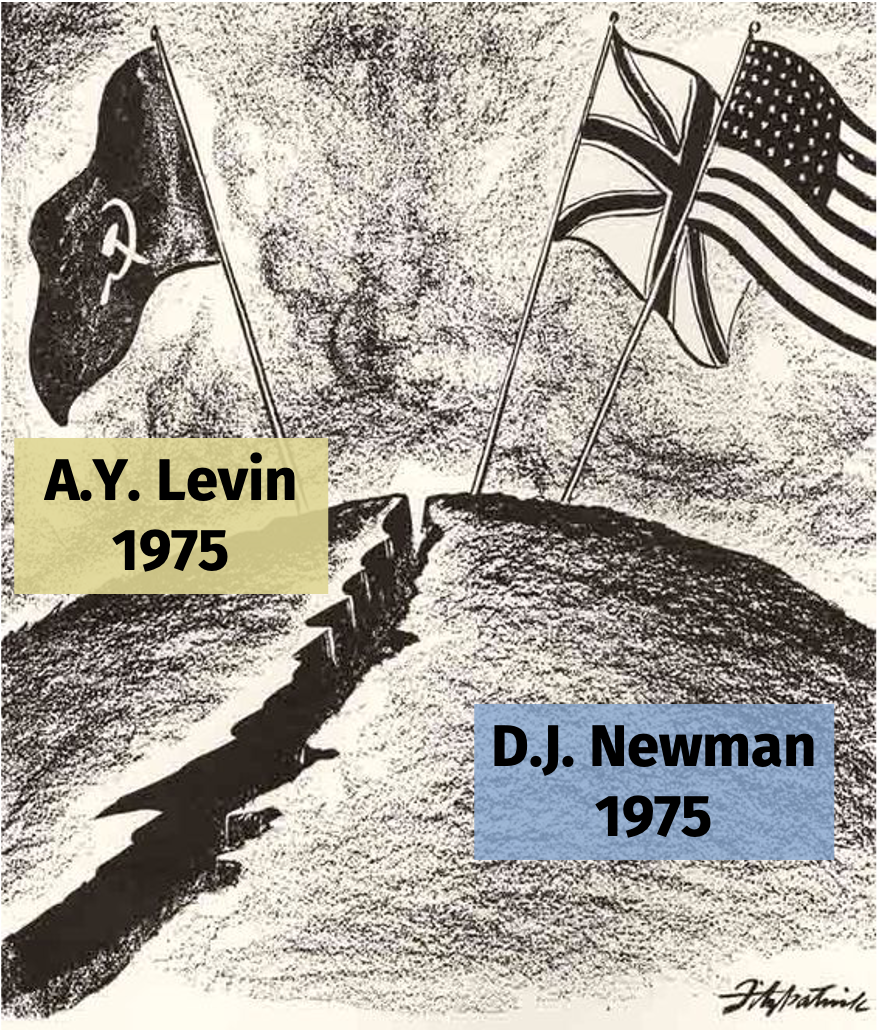
\includegraphics[width=.4\textwidth]{cog_proof.png}
\end{center}

\vspace{-.5em}
Not used in practice (we will discuss why) but the basic idea underlies many popular algorithms.
\end{frame}

\begin{frame}[t]
	\frametitle{center of gravity method}
	\textbf{A few basic ingredients:}

	1. The center-of-gravity of a convex set $\mathcal{S}$ is defined as:
	\begin{align*}
		c = \frac{\int_{x\in \mathcal{S}} x\, dx}{\vol(\mathcal{S})} =  \frac{\int_{x\in \mathcal{S}} x\, dx}{\int_{x\in \mathcal{S}} 1\, dx}
	\end{align*}

	2. For two convex sets $\mathcal{A}$ and $\mathcal{B}$, $\mathcal{A}\cap \mathcal{B}$ is convex. Proof by picture:
\end{frame}



\begin{frame}[t]
	\frametitle{center of gravity method}
	\begin{center}
	Natural ``cutting plane'' method.
	\end{center}
\begin{columns}
	\begin{column}{.6\textwidth}
		\begin{itemize}
			\item $\mathcal{S}_1 = \mathcal{S}$
			\item For $t = 1, \ldots, T:$
			\begin{itemize}
				\item \alert{$\bv{c}_t = \text{center of gravity of } \mathcal{S}_t$.}
				\item Compute $\nabla f(\bv{c}_t)$.
				\item $\mathcal{H} = \{\bv{x} \big\vert \langle \nabla f(\bv{c}_t), \bv{x}-\bv{c}_t\rangle \leq 0\}$.
				\item $\mathcal{S}_{t+1} = \mathcal{S}_{t} \cap H$
			\end{itemize}
			\item Return $\hat{\mathbf{x}} = \argmin_t f(\bv{c}_t)$
		\end{itemize}
	\end{column}
	\begin{column}{.35\textwidth}
	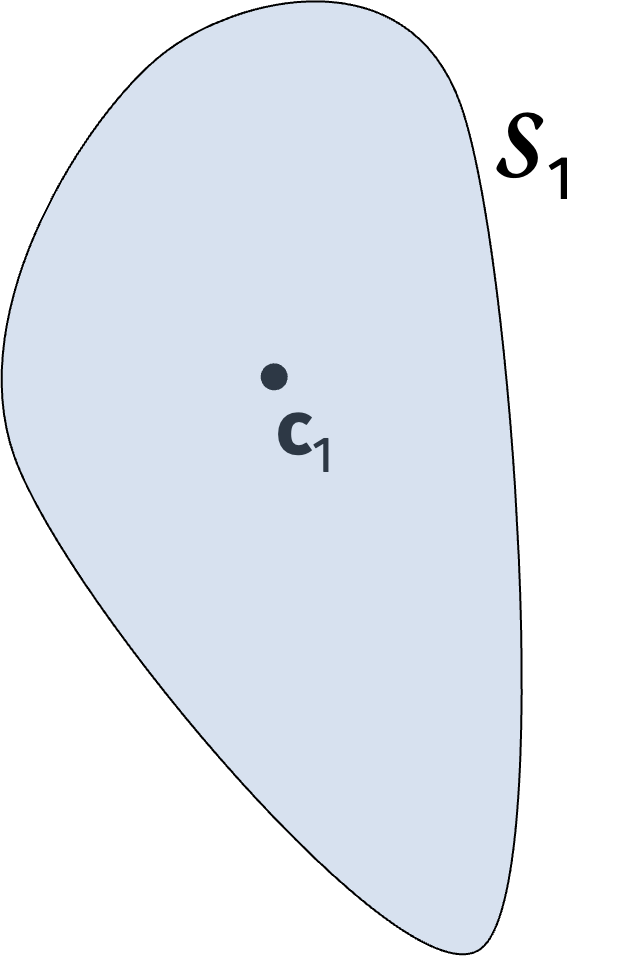
\includegraphics[width=\textwidth]{cog1.png}
\end{column}
\end{columns}
\end{frame}

\begin{frame}[t]
	\frametitle{center of gravity method}
	\begin{center}
		Natural ``cutting plane'' method.
	\end{center}
	\begin{columns}
		\begin{column}{.6\textwidth}
			\begin{itemize}
				\item $\mathcal{S}_1 = \mathcal{S}$
				\item For $t = 1, \ldots, T:$
				\begin{itemize}
					\item $\bv{c}_t = \text{center of gravity of } \mathcal{S}_t$.
					\item \alert{Compute $\nabla f(\bv{c}_t)$.}
					\item $\mathcal{H} = \{\bv{x} \big\vert \langle \nabla f(\bv{c}_t), \bv{x}-\bv{c}_t\rangle \leq 0\}$.
					\item $\mathcal{S}_{t+1} = \mathcal{S}_{t} \cap H$
				\end{itemize}
				\item Return $\hat{\mathbf{x}} = \argmin_t f(\bv{c}_t)$
			\end{itemize}
		\end{column}
		\begin{column}{.35\textwidth}
			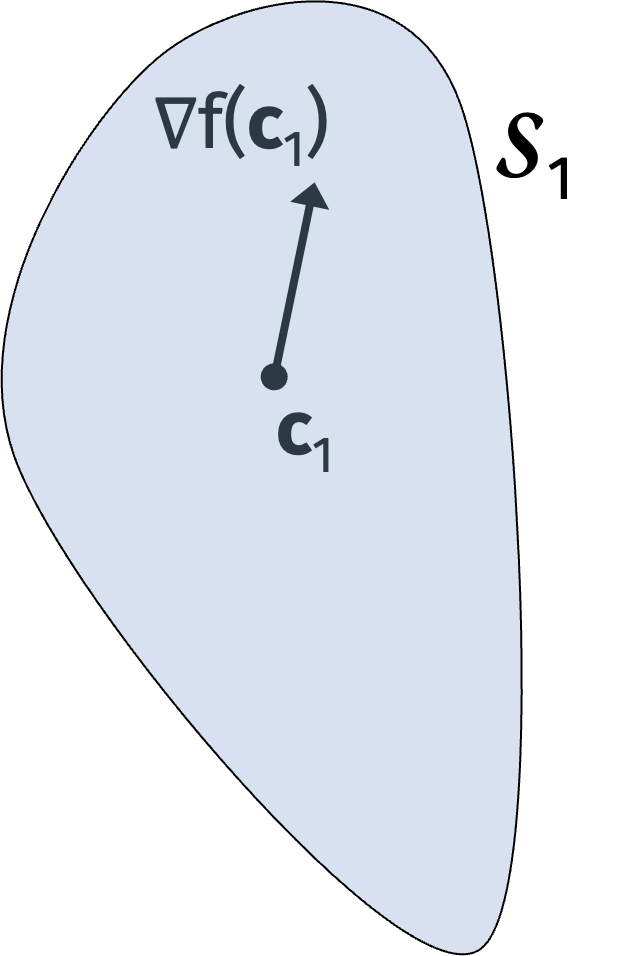
\includegraphics[width=\textwidth]{cog2.png}
		\end{column}
	\end{columns}
\end{frame}

\begin{frame}[t]
	\frametitle{center of gravity method}
	\begin{center}
		Natural ``cutting plane'' method.
	\end{center}
	\begin{columns}
		\begin{column}{.6\textwidth}
			\begin{itemize}
				\item $\mathcal{S}_1 = \mathcal{S}$
				\item For $t = 1, \ldots, T:$
				\begin{itemize}
					\item $\bv{c}_t = \text{center of gravity of } \mathcal{S}_t$.
					\item {Compute $\nabla f(\bv{c}_t)$.}
					\item \alert{$\mathcal{H} = \{\bv{x} \big\vert \langle \nabla f(\bv{c}_t), \bv{x}-\bv{c}_t\rangle \leq 0\}$.}
					\item \alert{$\mathcal{S}_{t+1} = \mathcal{S}_{t} \cap H$}
				\end{itemize}
				\item Return $\hat{\mathbf{x}} = \argmin_t f(\bv{c}_t)$
			\end{itemize}
		\end{column}
		\begin{column}{.6\textwidth}
			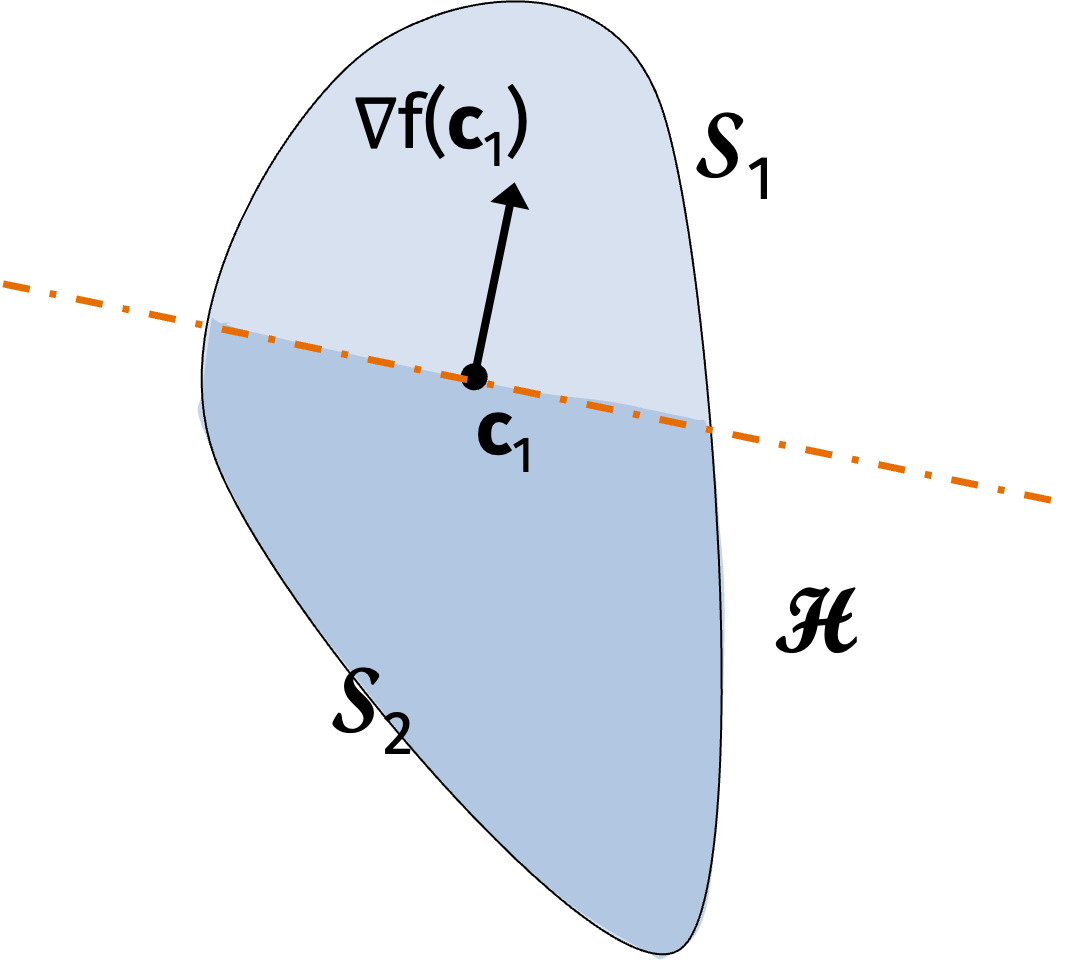
\includegraphics[width=\textwidth]{cog3.png}
		\end{column}
	\end{columns}
\end{frame}

\begin{frame}[t]
	\frametitle{center of gravity method}
	Intuitively, why does it make sense to search in $\mathcal{S}_t \cap \mathcal{H}$ where:
	\begin{align*}
		\mathcal{H} = \{\bv{x} \big\vert \langle \nabla f(\bv{c}_t), \bv{x}-\bv{c}_t\rangle \leq 0\}?
	\end{align*}
	\begin{center}
		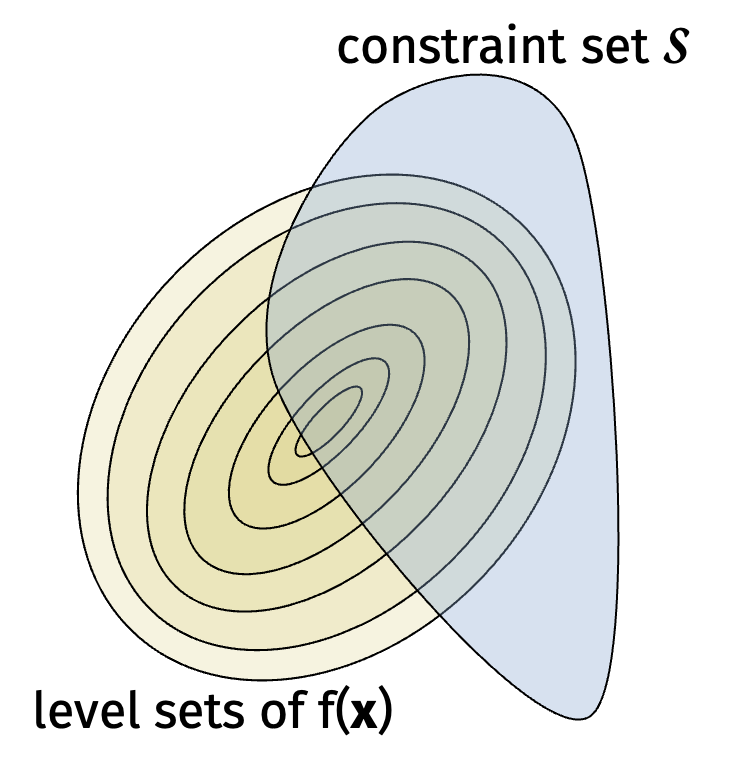
\includegraphics[width=.55\textwidth]{level_sets_constrained.png}
	\end{center}

\end{frame}

\begin{frame}[t]
	\frametitle{center of gravity method}
	Intuitively, why does it make sense to search in $\mathcal{S}_t \cap \mathcal{H}$ where:
	\begin{align*}
		\mathcal{H} = \{\bv{x} \big\vert \langle \nabla f(\bv{c}_t), \bv{x}-\bv{c}_t\rangle \leq 0\}?
	\end{align*}
	
	\begin{columns}
		\begin{column}{.45\textwidth}
			By convexity, 
			\begin{align*}
				f(\bv{y}) &\geq f(\bv{c}_t) +  \langle\nabla f(\bv{c}_t), \bv{y}-\bv{c}_t\rangle.
			\end{align*}

			If $\bv{y} \notin \{\mathcal{S}_t \cap \mathcal{H}\}$ then $\langle\nabla f(\bv{c}_t), \bv{y}-\bv{c}_t\rangle$ is negative, so $f(\bv{y}) > f(\bv{c}_t)$. 
		\end{column}
		\begin{column}{.55\textwidth}
			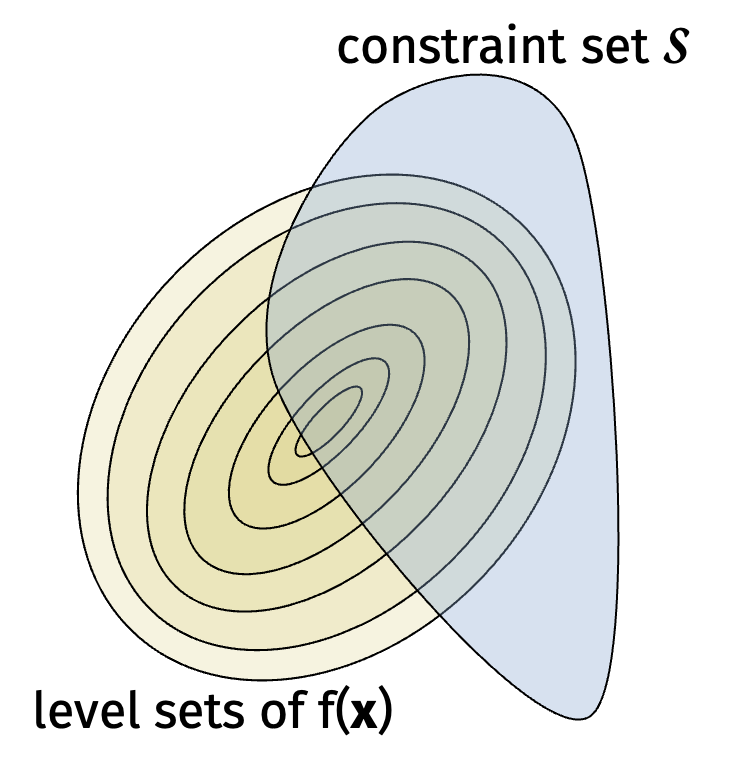
\includegraphics[width=\textwidth]{level_sets_constrained.png}
		\end{column}
	\end{columns}
	
\end{frame}

\begin{frame}[t]
	\frametitle{convergence theorem}
	\begin{theorem}[Center-of-Gravity Convergence]
		Let $f$ be a convex function with values in $[-B,B]$.
		Let $\hat{\bv{x}}$ be the output of the center-of-gravity method run for $T$ iterations. Then:
		\begin{align*}
			f(\hat{\bv{x}}) - f(\bv{x}^*) \leq 2B \left(1-\frac{1}{e}\right)^{T/d} \leq 2B e^{-T/3d}.
		\end{align*}
	\end{theorem}
	If we set $T = 3d\log(2B/\epsilon)$, then $f(\hat{\bv{x}}) - f(\bv{x}^*) \leq \epsilon$. 
\end{frame}

\begin{frame}[t]
	\frametitle{key geometric tool}
	Want to argue that, at every step of the algorithm, we ``cut off'' a large portion of the convex set we are searching over:
	
	\begin{center}
		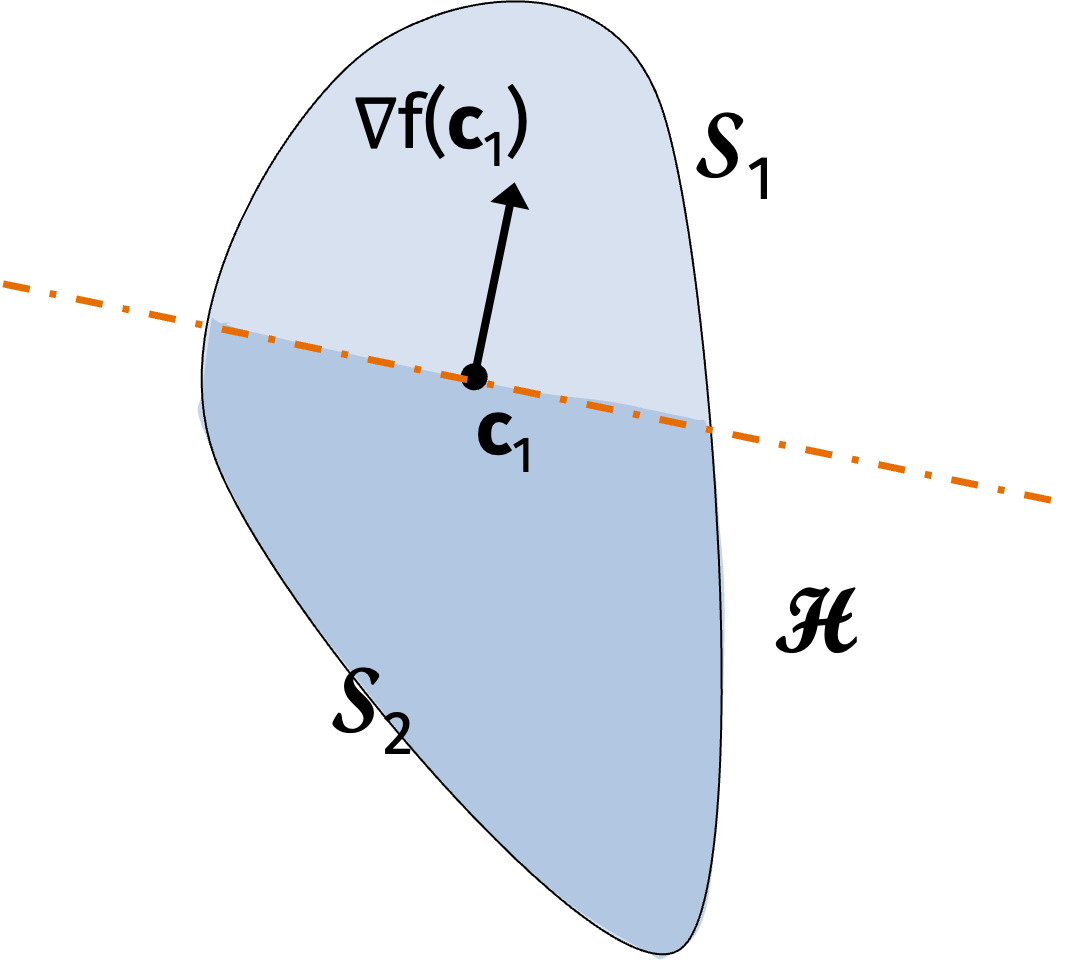
\includegraphics[width=.5\textwidth]{cog3.png}
	\end{center}
\end{frame}

\begin{frame}[t]
	\frametitle{key geometric tool}
	\begin{theorem}[Gr\"{u}nbaum's Theorem]
		For any convex set $\mathcal{S}$ with center-of-gravity $\bv{c}$, and any halfspace 	$\mathcal{Z} = \{\bv{x} \big\vert \langle \bv{a}, \bv{x}-\bv{c}\rangle \leq 0\}$ then:
		\begin{align*}
			\frac{\vol(\mathcal{S} \cap \mathcal{Z})}{\vol(\mathcal{S})}\geq \frac{1}{e} \approx .368
		\end{align*}
	\end{theorem}

\end{frame}

\begin{frame}[t]
	\frametitle{key geometric tool}
	Want to argue that, at every step of the algorithm, we ``cut off'' a large portion of the convex set we are searching over.
	
	\begin{theorem}[Gr\"{u}nbaum's Theorem]
		For any convex set $\mathcal{S}$ with center-of-gravity $\bv{c}$, and any halfspace 	$\mathcal{Z} = \{\bv{x} \big\vert \langle \bv{a}, \bv{x}-\bv{c}\rangle \leq 0\}$ then:
		\begin{align*}
			\frac{\vol(\mathcal{S} \cap \mathcal{Z})}{\vol(\mathcal{S})}\geq \frac{1}{e} \approx .368
		\end{align*}
	\end{theorem}
	
	Let $\mathcal{Z}$ be the compliment of $\mathcal{H}$ from the algorithm. Then we cut off at least a $1/e$ fraction of the convex body on every iteration.  
	
	\textbf{Corollary:} After $t$ steps, $\vol(\mathcal{S}_t) \leq \left(1-\frac{1}{e}\right)^t\vol(\mathcal{S})$.
\end{frame}

\begin{frame}
	\frametitle{convergence proof}
	Let $\delta$ be a small parameter to be chosen later. 
	
	Let $\mathcal{S}^{\delta} = \{(1-\delta)\bv{x}^* + \delta\bv{x} \hspace{.2em}\big\vert \hspace{.2em} \text{for } \bv{x}\in \mathcal{S} \}$.
	
	\begin{center}
	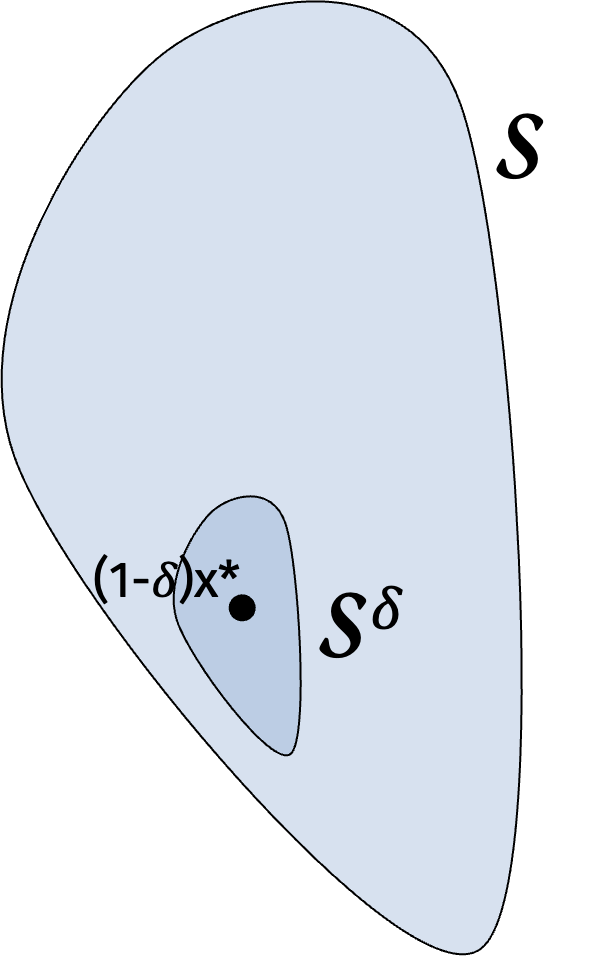
\includegraphics[width=.3\textwidth]{smallbody.png}
	\end{center}
	\textbf{Claim:} Every point $\bv{y}$ in $\mathcal{S}^{\delta}$ has good function value.
\end{frame}
\begin{frame}
	\frametitle{convergence proof}
	\begin{columns}
		\begin{column}{.3\textwidth}
		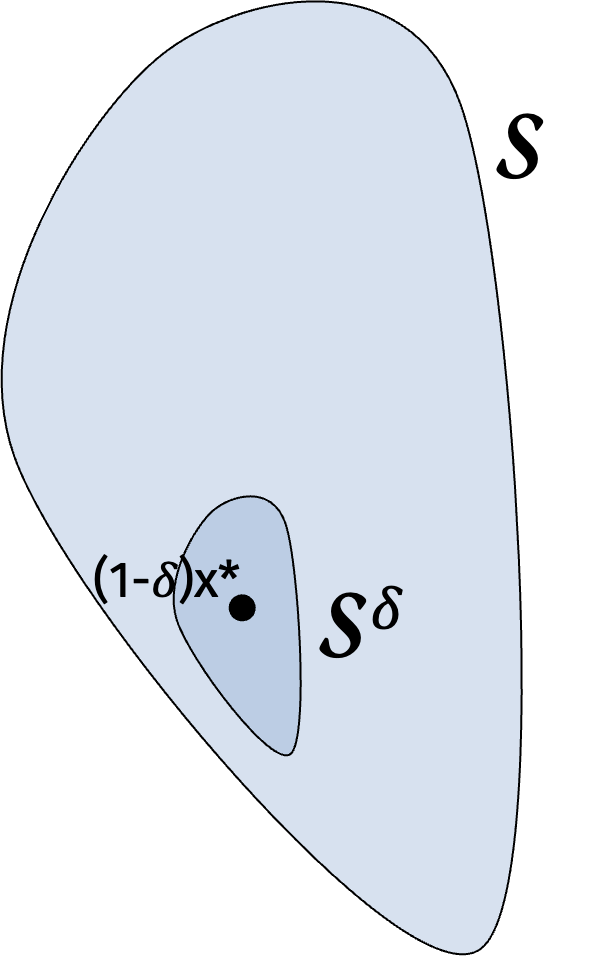
\includegraphics[width=\textwidth]{smallbody.png}
		\end{column}
		\begin{column}{.7\textwidth}
		For any $\bv{y} \in \mathcal{S}^\delta$:	
		\begin{align*}
			f(\bv{y}) &= f\left((1-\delta)\bv{x}^* + \delta \bv{x}\right) \\
			&\leq (1-\delta) f(\bv{x}^*) + \delta f(\bv{x})\\
			& \leq f(\bv{x}^*) - \delta f(\bv{x}^*)  + \delta f(\bv{x})\\
			&\leq f(\bv{x}^*)  + 2B\delta.
		\end{align*}
	\end{column}
	\end{columns}
\end{frame}

\begin{frame}
	\frametitle{convergence proof}
	\begin{columns}
		\begin{column}{.4\textwidth}
			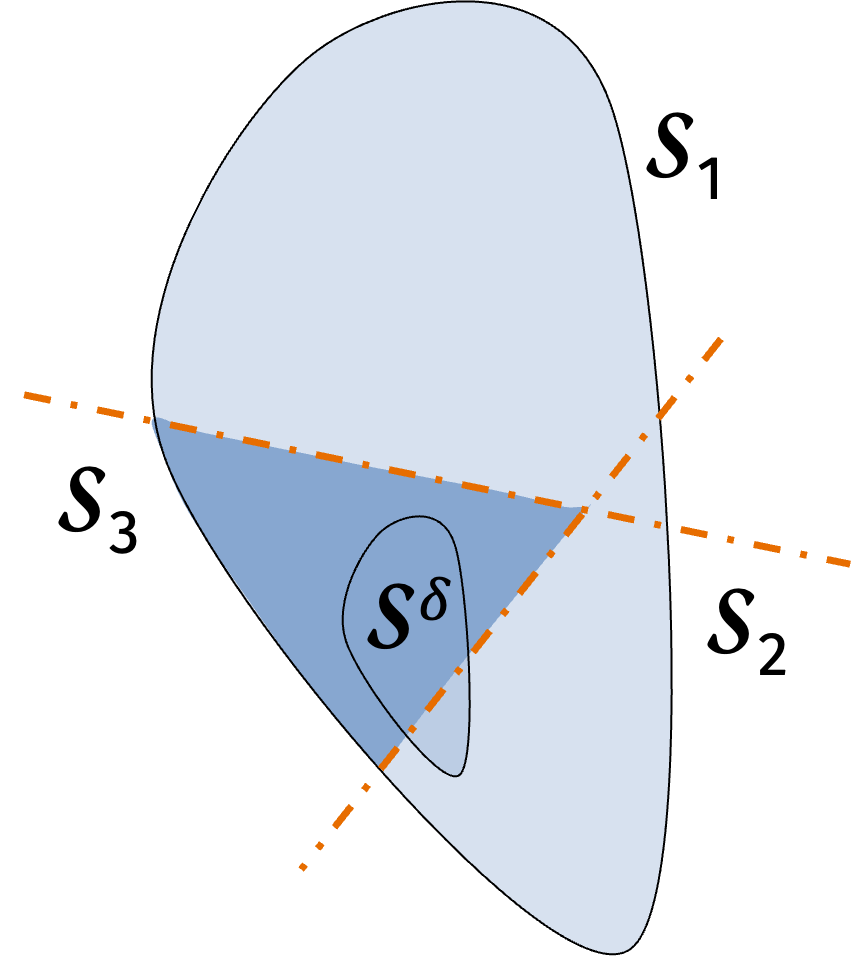
\includegraphics[width=\textwidth]{cut_off.png}
		\end{column}
		\begin{column}{.6\textwidth}
			\vspace{.5em}
			
			We also have: $\vol(\mathcal{S}^\delta) = \delta^d \vol(\mathcal{S}).$
			
			\vspace{1em}
			Set $\delta = \left(1-\frac{1}{e}\right)^{T/d}$. After $T$ steps, $\vol(\mathcal{S}_t) \leq \left(1-\frac{1}{e}\right)^{T} = \vol(\mathcal{S}^\delta)$.  
			
			\vspace{1em}
			Either $S_t$ exactly equals $S^{\delta}$, in which case our next centroid gives error $\leq 2B\delta$.
			
			\vspace{1em} Or we must have ``chopped off'' at least one point $\bv{y}$ in $\mathcal{S}^\delta$ by the time we reach step $T$. 
			\vspace{1em}
			
		\end{column}
	\end{columns}
\end{frame}

\begin{frame}
	\frametitle{convergence proof}
	\begin{columns}
		\begin{column}{.4\textwidth}
			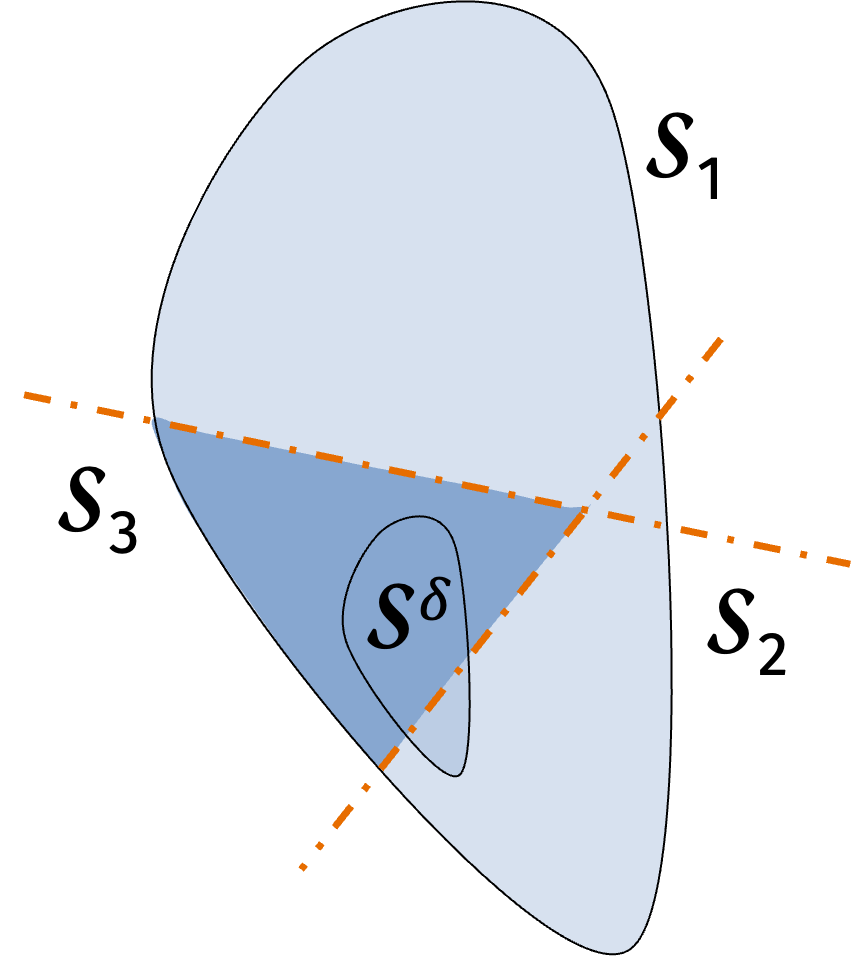
\includegraphics[width=\textwidth]{cut_off.png}
		\end{column}
		\begin{column}{.6\textwidth}
			\vspace{.5em}
			\textbf{Claim:} If we ``chopped off'' at least one point $\bv{y}$ in $\mathcal{S}^\delta$ by the time we reach step $T$ then for some centroid $\bv{c}_1, \ldots, \bv{c}_t$, $f(\bv{c}_t) < 2B\delta$. 
			\vspace{1em}
			
			\textbf{Proof:} 
			\begin{align*}
							2B\delta \geq f(\bv{y}) &\geq f(\bv{c}_t) +  \langle\nabla f(\bv{c}_t), \bv{y}-\bv{c}_t\rangle\\ &> f(\bv{c}_t).
			\end{align*}
		
			Algorithm returns $\argmin_{\bv{c}_i} f(\bv{c}_i)$.

		\end{column}
	\end{columns}
\end{frame}



\begin{frame}[t]
	\frametitle{convergence theorem}
	\begin{theorem}[Center-of-Gravity Convergence]
		Let $f$ be a convex function with values in $[-B,B]$.
		Let $\hat{\bv{x}}$ be the output of the center-of-gravity method run for $T$ iterations. Then:
		\begin{align*}
			f(\hat{\bv{x}}) - f(\bv{x}^*) \leq 2B \left(1-\frac{1}{e}\right)^{T/d} \leq 2B e^{-T/3d}.
		\end{align*}
	\end{theorem}
	If we set $T = O\left(d\log(B/\epsilon)\right)$, then $f(\hat{\bv{x}}) - f(\bv{x}^*) \leq \epsilon$. 

In terms of \emph{gradient-oracle} complexity, this is essentially optimal. So why isn't the algorithm used?
\end{frame}


\begin{frame}[t]
		\frametitle{centroid computation}
		\textbf{In general computing the centroid is hard.} \#P-hard even when when $\mathcal{S}$ is an intersection of half-spaces (a polytope).
		
		Even if the problem isn't hard for your starting convex body $\mathcal{S}$, it likely will become hard for $\mathcal{S} \cap \mathcal{H}_1  \cap \mathcal{H}_2 \cap \mathcal{H}_3 \ldots$. 
		
		So while the \emph{oracle complexity} of dimension-dependent optimization was settled in the 70s, a number of basic questions in terms of \emph{computational complexity.}

		\vspace{1em}
		We will discuss how to obtain a computationally efficient version of the center-of-gravity method called the \textbf{ellipsoid method.} This method is most famous for giving the first polynomial time algorithm for linear programming. 
\end{frame}

\begin{frame}[standout]
	\begin{center}
		\large break
	\end{center}
\end{frame}

\begin{frame}[t]
	\frametitle{linear programming}
	\textbf{Linear programs} (LPs) are one of the most basic convex constrained, convex optimization problems:
	
	Let $\bv{c}\in \R^d, \bv{b}\in \R^n, \bv{A}\in \R^{n\times d}$ be fixed vectors that define the problem, and let $\bv{x}$ be our variable parameter.
	\begin{align*}
	\min f(\bv{x}) &= \bv{c}^T\bv{x}\\
	\text{subject to } \bv{A}\bv{x} &\geq \bv{b}.
	\end{align*}
	
Think about $\bv{A}\bv{x} \geq \bv{b}$ as a union of half-space constraints:
\begin{align*}
	&\{\bv{x}: \bv{a}_1^T\bv{x} \geq {b}_1 \}\\
		&\{\bv{x}: \bv{a}_2^T\bv{x} \geq {b}_2 \}\\
			&\hspace{2.3em}\vdots\\
			&\{\bv{x}: \bv{a}_n^T\bv{x} \geq {b}_n \}
\end{align*}
	
\end{frame}

\begin{frame}[t]
	\frametitle{linear programming}
	\begin{align*}
		\min f(\bv{x}) &= \bv{c}^T\bv{x}\\
		\text{subject to } \bv{A}\bv{x} &\geq \bv{b}.
	\end{align*}
	
	\begin{center}
		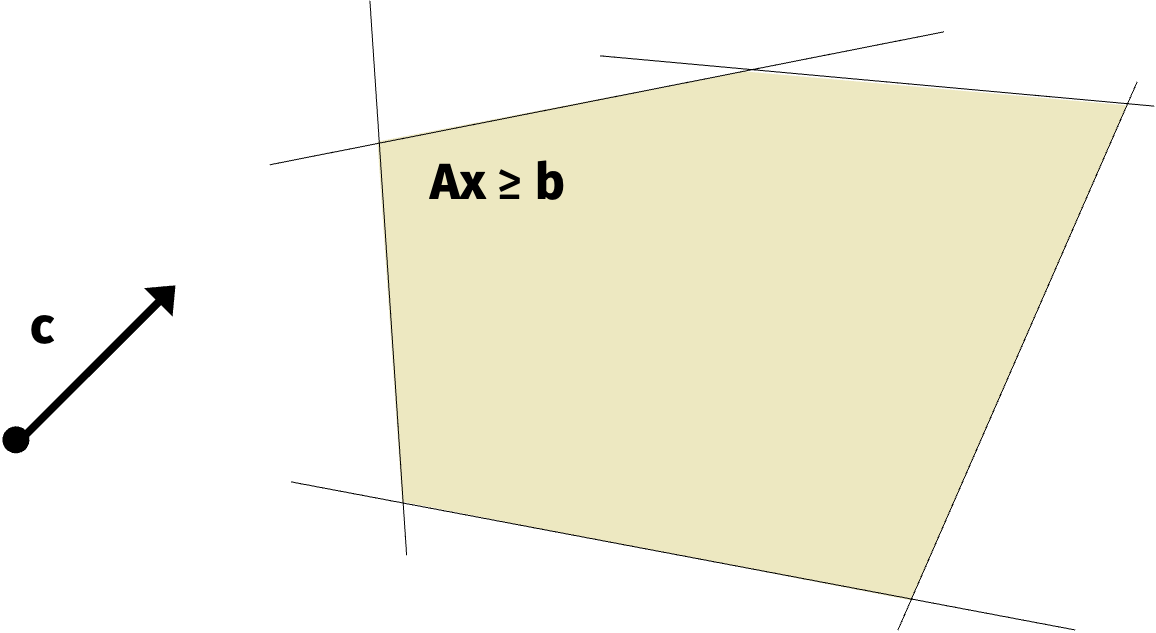
\includegraphics[width=.8\textwidth]{lpexample.png}
	\end{center}
\end{frame}

\begin{frame}
		\frametitle{linear programming applications}
	\begin{itemize}
		\item Classic optimization applications: industrial resource optimization problems were killer app in the 70s.
		\item Robust regression: $\min_{\bv{x}} \|\bv{A} \bv{x} - \bv{b}\|_1$. 
		\item $L1$ constrained regression: $\min_{\bv{x}} \|\bv{x}\|_1$ subject to $\bv{A}\bv{x} = \bv{b}$. Lots of applications in sparse recovery/compressed sensing.
		\item Solve $\min_{\bv{x}}\|\bv{A} \bv{x} - \bv{b}\|_{\infty}$.   
		\item Polynomial time algorithms for Markov Decision Processes. 
		\item \alert{\textbf{Many combinatorial optimization problems can be solved via \emph{LP relaxations}.}}
	\end{itemize}
\end{frame}

\begin{frame}[t]
	\frametitle{linear programming}
	\begin{theorem}[Khachiyan, 1979]
	Assume $n=d$. The \emph{ellipsoid method} solves any linear program with $L$-bit integer valued constraints in $O(n^4L)$ time. 
	\end{theorem}
Ellipsoid is a relatively simple center-of-gravity like method!
	\begin{center}
		
\includegraphics[width=\textwidth]{ellipsoidnews.png}
		Front page of New York Times, November 9, 1979.
	\end{center}
\end{frame}

\begin{frame}[t]
	\frametitle{problem simplification}
	\small
		\textbf{Simplifying the problem:}
		Given a convex set $\mathcal{K}$ via access to \emph{separation oracle} $S_\mathcal{K}$ for the set, determine if $\mathcal{K}$ is empty, or otherwise return any point $\bv{x}\in \mathcal{K}$. 
		\vspace{-2em}
		
		\begin{align*}
			\bv{S}_k(\bv{y}) = \begin{cases}
				\emptyset &\text{ if } \bv{y} \in \mathcal{K}. \\
				\text{separating hyperplane } (\bv{a},c) &\text{ if } \bv{y} \notin \mathcal{K}.
			\end{cases}
		\end{align*}
	
	Let $\mathcal{H} = \{\bv{x}: \bv{a}^T\bv{x} = c\}$.
	\vspace{-1em}
		\begin{center}
			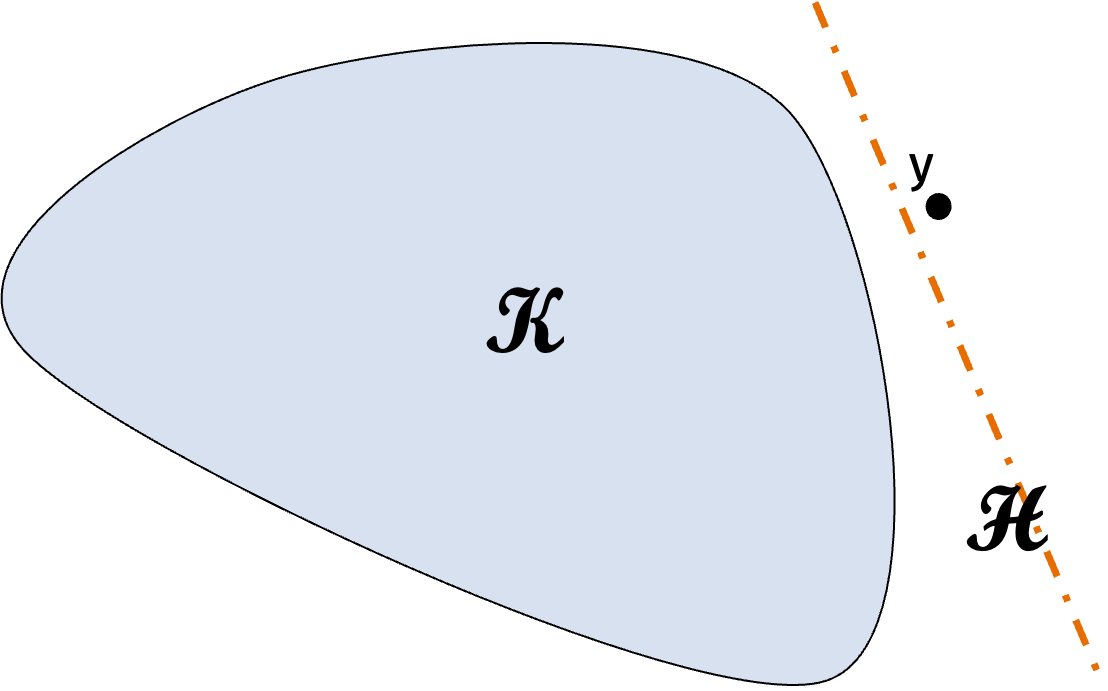
\includegraphics[width=.65\textwidth]{seperationoracle.png}
		\end{center}
	
\end{frame}

\begin{frame}[t]
	\frametitle{separation oracle}
	\textbf{Example:} How would you implement a separation oracle for a polytope $\{\bv{x}: \bv{A}\bv{x} \geq \bv{b}\}$. 
\end{frame}

\begin{frame}[t]
	\frametitle{from membership to optimization}
	\textbf{Original problem:} $\min_{\bv{x}\in \mathcal{S}} f(\bv{x})$.

	How to reduce to determining if a convex set $\mathcal{K}$ is empty or not?
	\begin{center}
	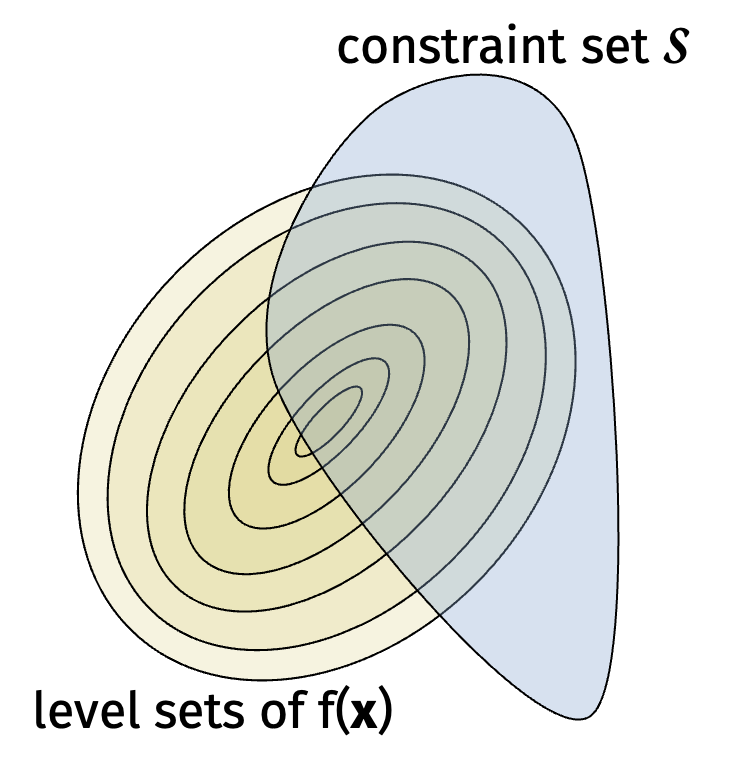
\includegraphics[width=.5\textwidth]{level_sets_constrained.png}
	\end{center}
	
\end{frame}

\begin{frame}[t]
	\frametitle{from membership to optimization}
	\textbf{Original problem:} $\min_{\bv{x}\in \mathcal{S}} f(\bv{x})$.

	How to reduce to determining if a convex set $\mathcal{K}$ is empty or not?
	\begin{center}
		\vspace{-1em}
	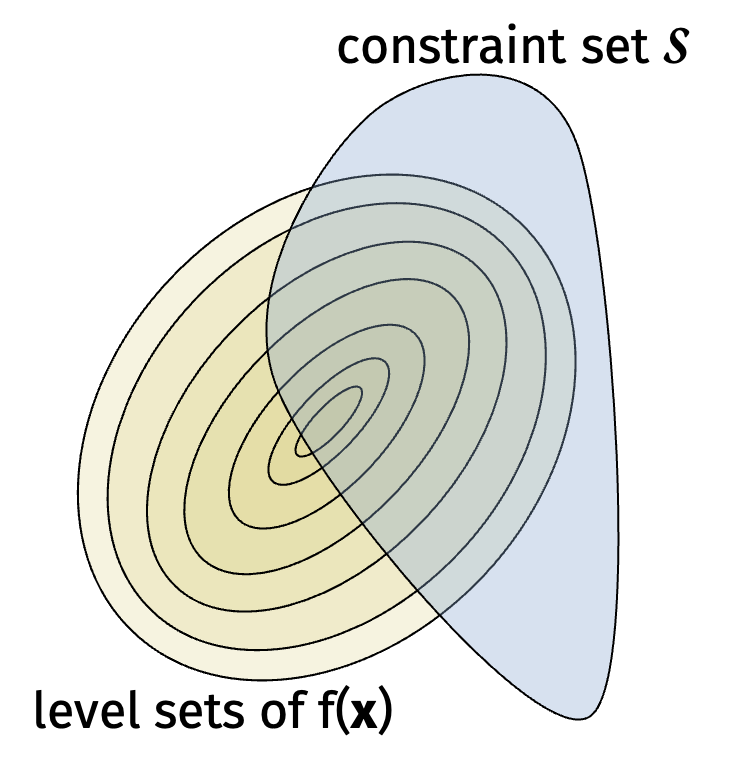
\includegraphics[width=.5\textwidth]{level_sets_constrained.png}
	\vspace{-1em}
	\end{center}
	
	\textbf{Binary search!} For a convex function $f(\bv{x})$, $\{\bv{x}: f(\bv{x}) \leq c\}$ is convex, and you can get a separation oracle via the gradient.
\end{frame}



\begin{frame}[t]
\frametitle{ellipsoid method sketch}
\textbf{Goal of ellipsoid algorithm:} Solve ``Is $\mathcal{K}$ empty or not?" given a separation oracle for $\mathcal{K}$ under the assumptions that:
\begin{enumerate}
	\item $\mathcal{K} \subset B(\bv{c}_R, R)$.
	\item If non-empty, $\mathcal{K}$ contains $B(\bv{c}_r, r)$ for some $r < R$. 
\end{enumerate}
\begin{center}
	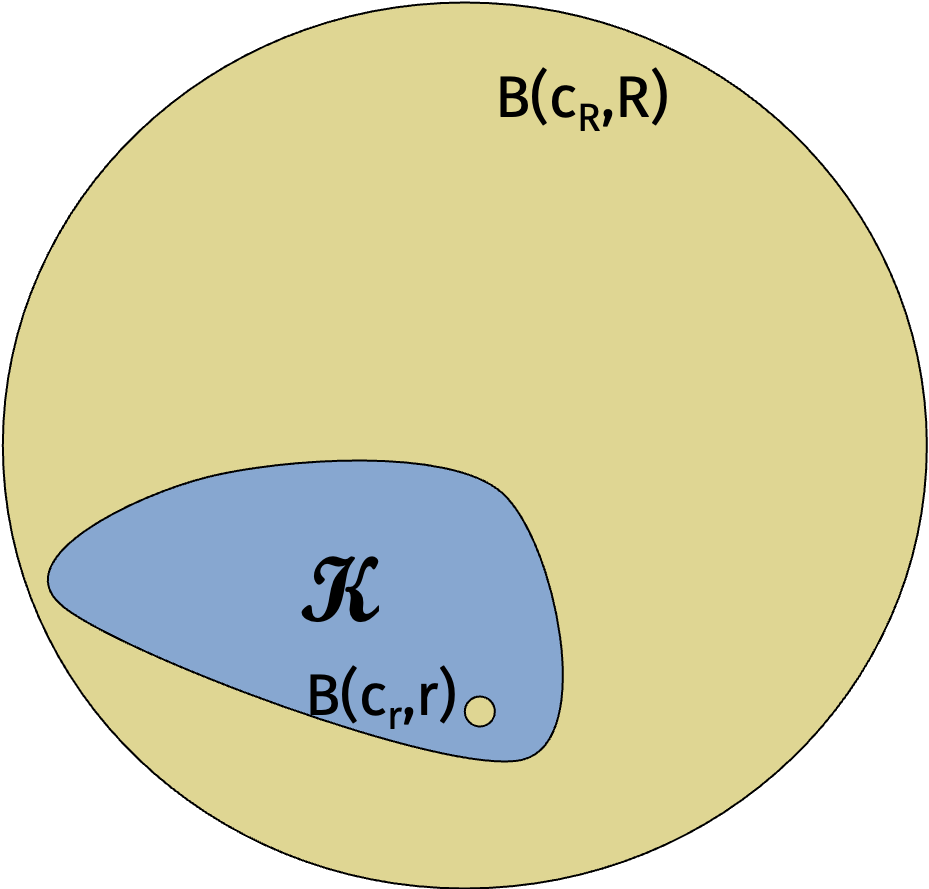
\includegraphics[width=.5\textwidth]{ellipsoid0.png}
\end{center}
	
\end{frame}

\begin{frame}[t]
	\frametitle{ellipsoid method sketch}
	Iterative method similar to center-of-gravity:
	\begin{enumerate}
		\item Check if center $\bv{c}_R$ of $B(\bv{c}_R, R)$ is in $\mathcal{K}$.
		\item If it is, we are done.
		\item  If not, cut search space in half, using separating hyperplane. 
	\end{enumerate}
	\begin{center}
		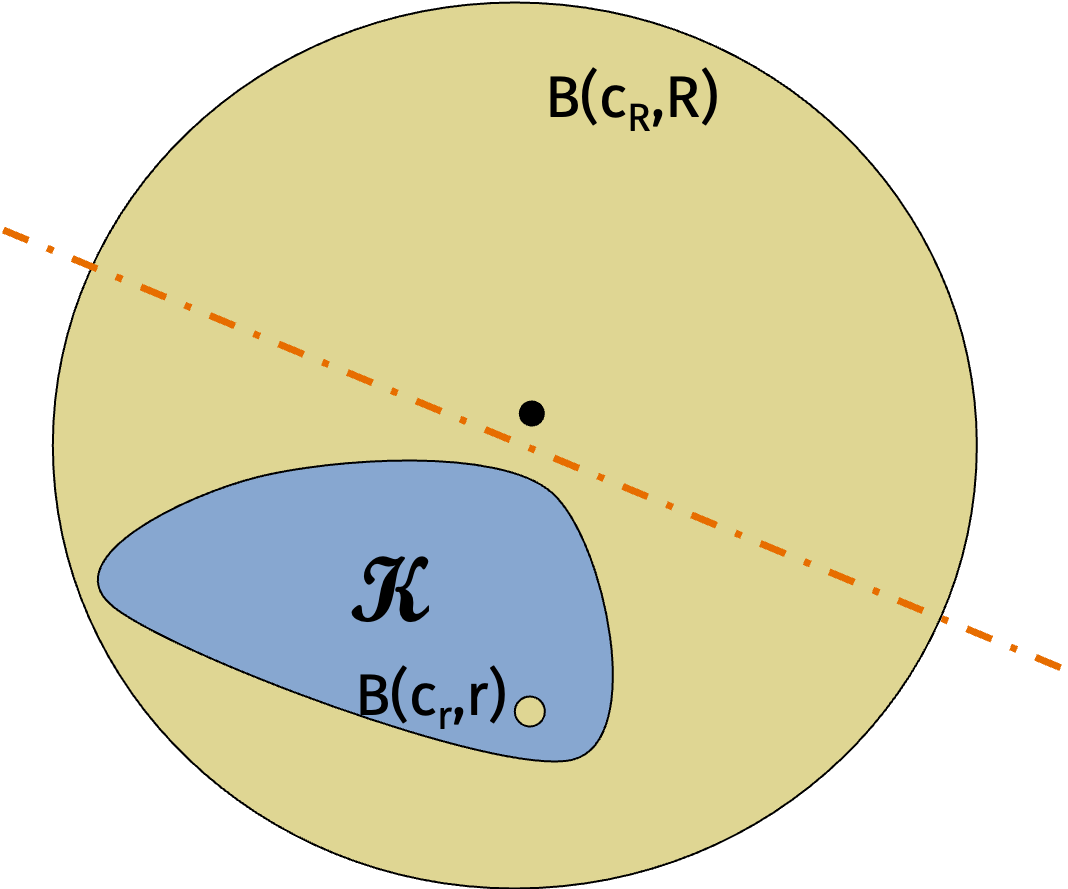
\includegraphics[width=.5\textwidth]{ellipsoid1.png}
	\end{center}
\end{frame}

\begin{frame}[t]
	\frametitle{ellipsoid method sketch}
	\textbf{Key insight:} Before moving on, approximate new search region by something that we can easily compute the centroid of. Specifically an ellipse!!
	\vspace{-1em}
	\begin{center}
		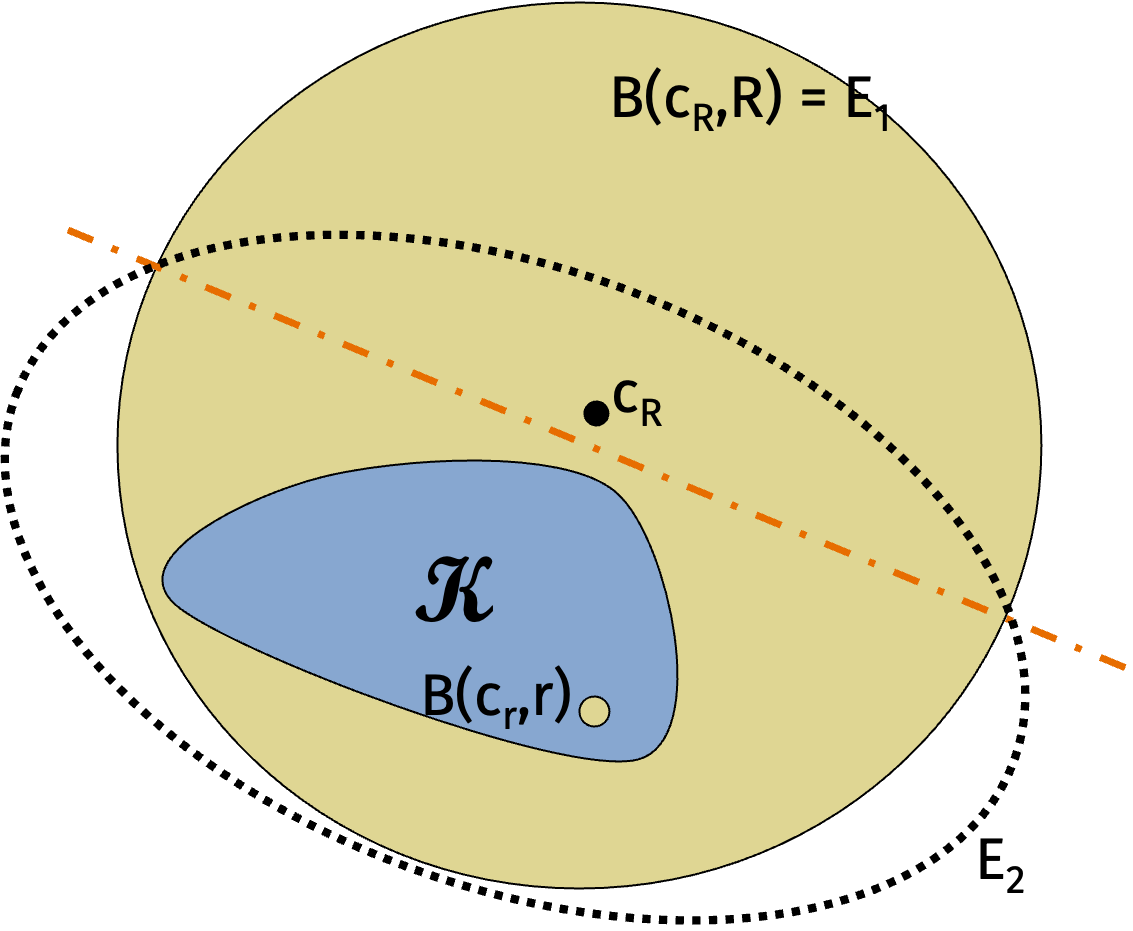
\includegraphics[width=.5\textwidth]{ellipsoid2.png}
	\end{center}
	\vspace{-1em}
Produce a sequence of ellipses that \emph{always contain} $\mathcal{K}$ and decrease in volume: $B(\bv{c}_R, R) = E_1, E_2, \ldots$. Once we get to an ellipse with volume $\leq B(\bv{c}_r, r)$, we know that $\mathcal{K}$ must be empty.
\end{frame}

\begin{frame}
		\frametitle{ellipse}
		An ellipse is a convex set of the form: $\{\bv{x}: \|\bv{A}(\bv{x} - \bv{c})\|_2^2 \leq \alpha\}$ for some constant $c$ and matrix $\bv{A}$. The center-of-mass is  $\bv{c}$. 
		\begin{center}
			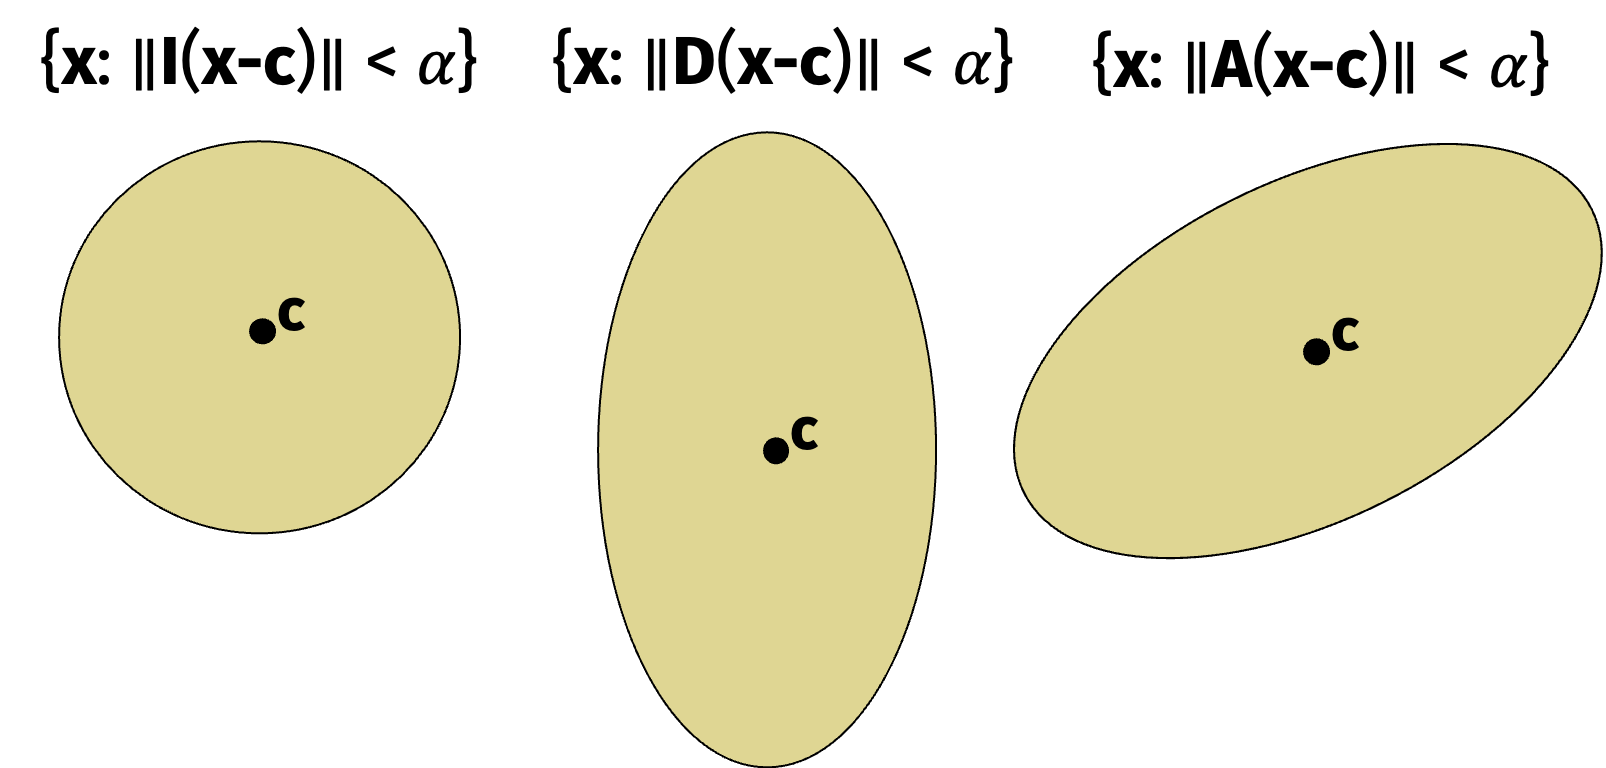
\includegraphics[width=\textwidth]{ellipses.png}
		\end{center}
	
	Often re-parameterized to say that the ellipse is all $\bv{x}$ with $\{\bv{x}: (\bv{x} - \bv{c})^T\bv{Q}^{-1}(\bv{x} - \bv{c})\leq 1\}$
\end{frame}

\begin{frame}
	\frametitle{ellipsoid update}
	There is a closed form solution for the equation of the smallest ellipse containing a given half-ellipse. I.e. let $\bv{E}_i$ have parameters $\bv{Q}_i,\bv{c}_i$ and consider the half-ellipse:
	\begin{align*}
		\bv{E}_i \cap \{\bv{x}: \bv{a}_i^T\bv{x} \leq \bv{a}_i^T\bv{c}_i\}. 
	\end{align*}
Then $\bv{E}_{i+1}$ is the ellipse with parameters:
\begin{align*}
	\bv{Q}_{i+1} &= \frac{d^2}{d^2 - 1}\left(\bv{Q}_{i} - \frac{2}{d+1} \bv{h}\bv{h}^T \right) & \bv{c}_{i+1}& = \bv{c}_{i} - \frac{1}{n+1}\bv{h},
\end{align*}
where $\bv{h} = \sqrt{\bv{a}_i^T\bv{Q}_i\bv{a}_i}\cdot \bv{a}_i$. 
	
\end{frame}


\begin{frame}[t]
	\frametitle{geometric observation}
	\textbf{Claim:} $\vol(E_{i+1}) \leq (1-\frac{1}{2d})\vol(E_i)$.
	
	\textbf{Proof:} Via reduction to the ``isotropic case''. I will post a proof on the course website if you are interested. 
	\vspace{-.5em}
	\begin{center}
		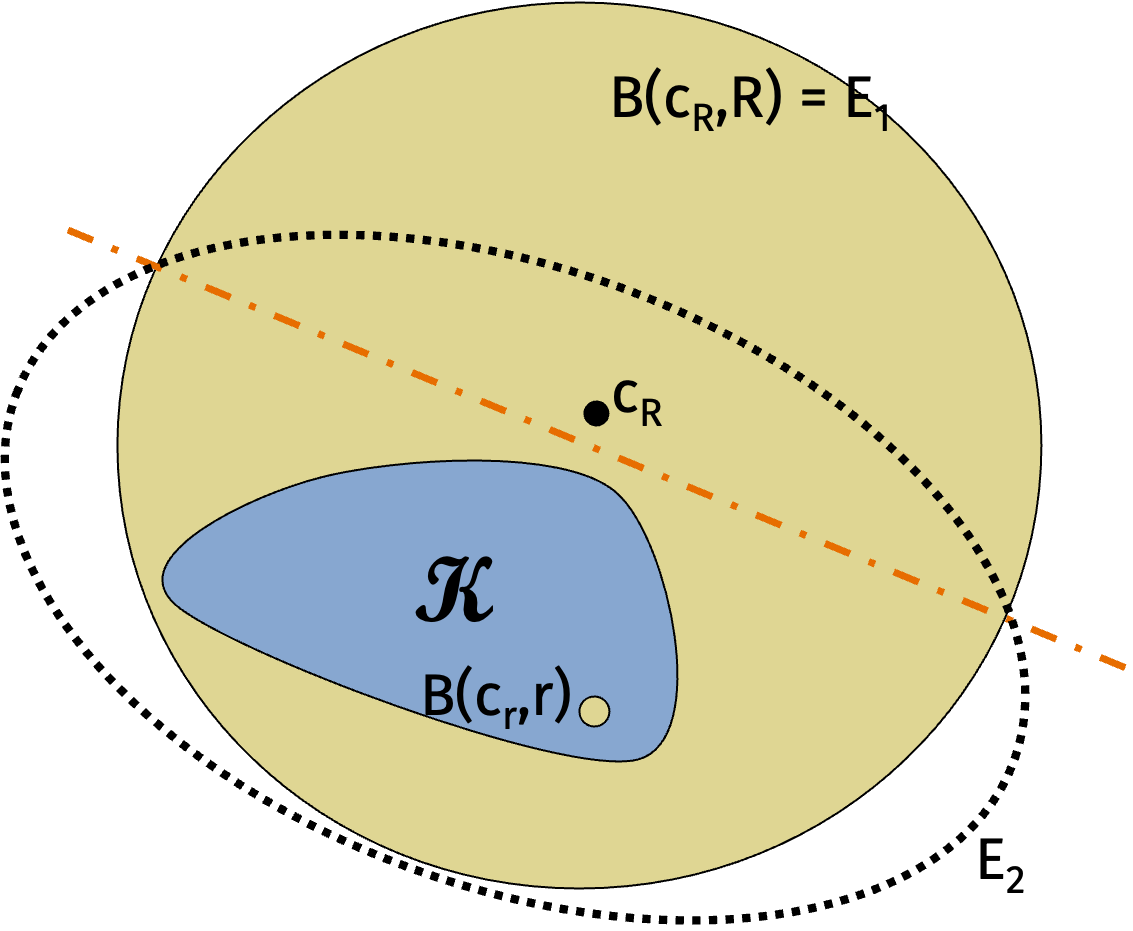
\includegraphics[width=.5\textwidth]{ellipsoid2.png}
	\end{center}
	\vspace{-.5em}
Not as good as the $(1-\frac{1}{e})$ constant-factor volume reduction we got from center-of-gravity, but still very good! 
\end{frame}


\begin{frame}[t]
	\frametitle{geometric observation}
	\textbf{Claim:} $\vol(E_{i+1}) \leq (1-\frac{1}{2d})\vol(E_i)$

	\begin{center}
		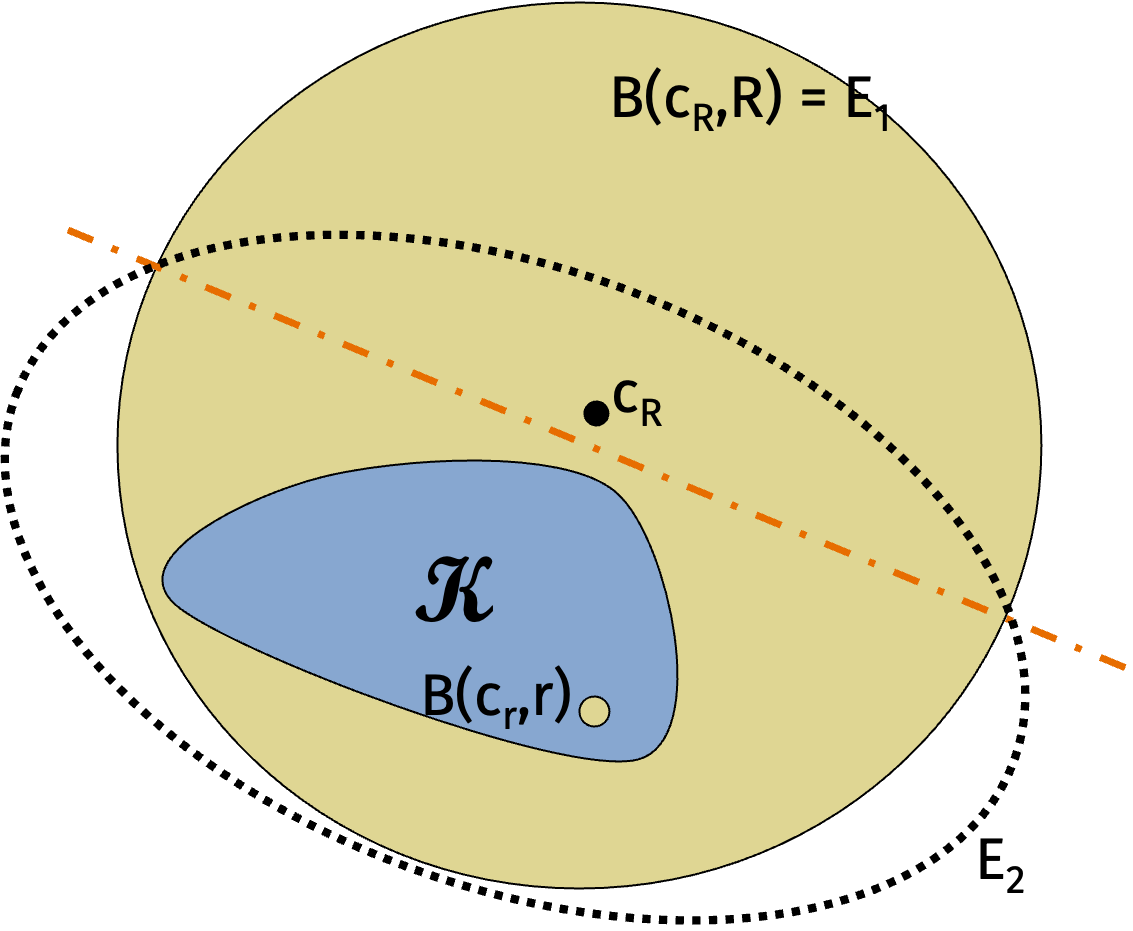
\includegraphics[width=.5\textwidth]{ellipsoid2.png}
	\end{center}
	\begin{center}
		After $O(d)$ iterations, we reduce the volume by a constant.
		
		In total require $O(d^2\log(R/r))$ iterations to solve the problem.
	\end{center}
\end{frame}

\begin{frame}[t]
	\frametitle{ellipsoid for LPs}
	\begin{theorem}[Khachiyan, 1979]
		Assume $n=d$. The \emph{ellipsoid method} solves any linear program with $L$-bit integer valued constraints in $O(n^4L)$ time. I.e. linear programming is in (weakly) polynomial time!
	\end{theorem}
The method works for any convex program. 

For LPs, we have an $O(nd)$ time separation oracle, and ellipsoid update take $O(d^2)$ time.

 Careful analysis of the binary search method, how to set $B_r$ and $B_R$, etc. leads to the final runtime bound. 
\end{frame}

\begin{frame}[t]
	\frametitle{interior point methods}
	\begin{theorem}[Karmarkar, 1984]
		Assume $n=d$. The \emph{interior point method} solves any linear program with $L$-bit integer valued constraints in $O(n^{3.5}L)$ time. 
	\end{theorem}
	\begin{center}
	
\includegraphics[width=.7\textwidth]{interiornews.png}
	
			Front page of New York Times, November 19, 1984.
	\end{center}
\end{frame}

\begin{frame}[t]
	\frametitle{interior point methods}
	Will post lecture notes on the website (optional reading).
	\begin{center}
			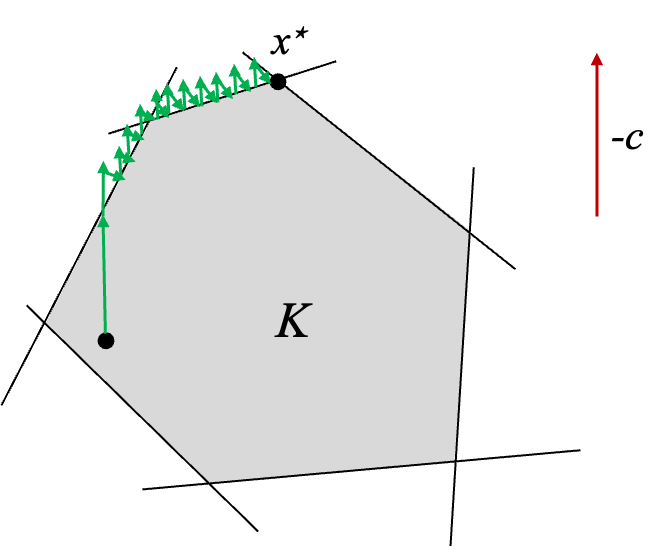
\includegraphics[width=.6\textwidth]{projected_gradient.png}
			
			Projected Gradient Descent Optimization Path
	\end{center}

\end{frame}

\begin{frame}[t]
	\frametitle{interior point methods}
	Will post lecture notes on the website (optional reading).
	\begin{center}
		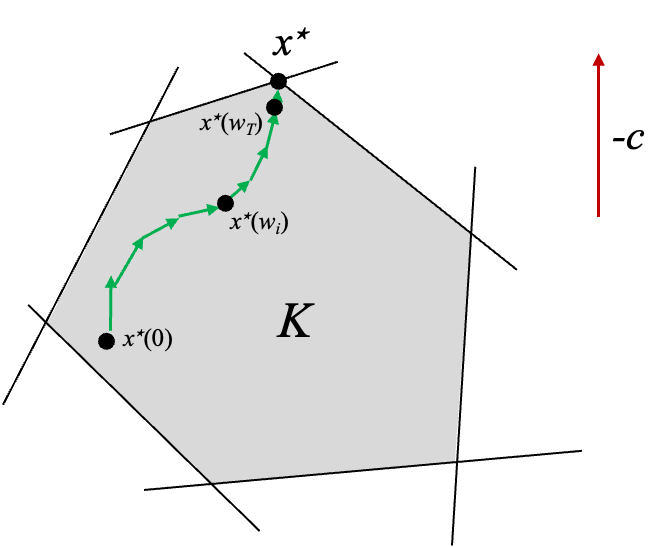
\includegraphics[width=.6\textwidth]{interior_point.png}
		
		Ideal Interior Point Optimization Path
	\end{center}
	
\end{frame}

\begin{frame}[t]
	\frametitle{polynomial time linear programming}
	Both results had a huge impact on the theory of optimization, although at the time neither the ellipsoid method or interior point method were faster than a heuristic known at the Simplex Method. 
	
	These days, improved interior point methods compete with and often outperform simplex. 
	
\end{frame}

% \begin{frame}[standout]
% 	\begin{center}
% 			\large lp relaxation
% 		\end{center}
% \end{frame}

% \begin{frame}
% 	\frametitle{set cover problem}	
% 	Given:
% 	\begin{itemize}
% 		\item $n$ ground elements $\{1,\ldots,n\}$
% 		\item $m$ sets $S_1,S_2,\ldots,S_m$ where $S_j \subseteq \{1,\ldots,n\}$
% 		\item non-negative weights $c_1, \ldots, w_m\geq 0$
% 	\end{itemize}
	
% 	\vspace{2em}
	
% 	Find:
% 	\begin{align*}
% 		\min_{Z \subseteq \{1,\ldots,m\}}
% 		\sum_{j \in Z} c_j
% 		\hspace{2em}
% 		\textnormal{ subject to }
% 		\hspace{2em}
% 		\cup_{j \in Z} S_j = \{1,\ldots,n\}.
% 	\end{align*}

% \begin{center}
% \textbf{\alert{This is an NP-Complete combinatorial optimization problem! Likely impossible to find an efficient \emph{exact} algorithm.}}
% \end{center}
% \end{frame}

% \begin{frame}
% 	\frametitle{applications}
% 	\begin{itemize}
% 		\item Finding efficient sets of test cases for code testing and verification.
% 		\item Complex employee shift scheduling problems (e.g. in the airline industry).
% 		\item Motif selection in computational biology.
% 	\end{itemize}
% \end{frame}

% \begin{frame}
% 	\frametitle{application: vertex cover}
	
% 	Given:
% 	\begin{itemize}
% 		\item ground elements are edges
% 		\item sets are nodes so
% 		\begin{align*}
% 			S_j = \{ \textnormal{edges adjacent to
% 				$j$th node}\}
% 		\end{align*}
% 		\item Could have $c_j=1$ for all $j\in 1, \ldots, m$ or could have different costs per node.
% 	\end{itemize}
% 	\vspace{2em}
	
% 	What vertices should we choose so that all
% 	edges are connected to at least one chosen
% 	vertex?
% \end{frame}

% \begin{frame}
% 	\frametitle{linear programming}
% 	Let $\mathbf{x} \in \R^m$ be a vector
% 	of decision variables, $\mathbf{c}$ be a cost vector, and $\mathbf{b} \in \R^n$
% 	be a vector of constraints. As before a linear program has the form
% 	the linear programs is:
% 	\begin{align*}
% 		\textnormal{Minimize} \hspace{1em}
% 		\mathbf{c^T x} \hspace{1em}
% 		&\textnormal{ subject to } \hspace{1em}
% 		\mathbf{Ax \geq b}, \hspace{1em}
% %		\mathbf{x} \geq 0 \hspace{1em}
% 	\end{align*}
	
% 	\vspace{2em}	
	
% 	\textbf{Goal:} Show that set cover can be written as a linear program, except with the additional constraint that $\bv{x}$ is a \emph{binary} random vector. This is called an  \textbf{\alert{integer linear program}}.
% \end{frame}

% \begin{frame}
% 	\frametitle{lp for set cover: objective}
	
% 	Let $x_j = 1$ iff $j \in Z$. $0$ otherwise
	
% 	The objective is to minimize the sum of weights
% 	in $Z$:
	
% 	\begin{align*}
% 		\min_{Z\subseteq \{1,\ldots,m\}} \sum_{j \in Z} c_j
% 		\hspace{1em} \Leftrightarrow \hspace{1em}
% 		\min_{\mathbf{x}} \sum_{j=1}^m c_j x_j
% 		\hspace{1em} \Leftrightarrow \hspace{1em}
% 		\min_{\mathbf{x}} \mathbf{c^T x}
% 	\end{align*}
% \end{frame}

% \begin{frame}
% 	\frametitle{lp for set cover: constraint}
	
% 	The constraint is that $C$
% 	covers the ground elements. I.e. for all $i \in 1,\dots, n$, we should have:
	
% 	\begin{align*}
% 		i \in \cup_{j \in Z} S_j
% 		\hspace{1.5em} \Leftrightarrow \hspace{1em}
% 		\sum_{j:i \in S_j}^m x_j \geq 1 
% 		\hspace{1.5em} \Leftrightarrow \hspace{1em}
% 		\mathbf{A x \geq c}
% 	\end{align*}	
	
% 	\textbf{Question:} What are $\mathbf{A}$ and $\mathbf{b}$?
	
% \end{frame}

% \begin{frame}
% 	\frametitle{lp for set cover: statement}
% 	\begin{align*}
% 		\textnormal{Minimize} \hspace{1em}
% 		\mathbf{c^T x} \hspace{1em}
% 		&\textnormal{ subject to } \hspace{1em}
% 		\mathbf{Ax \geq b}, \hspace{1em} \bv{x}\in \{0,1\}^m		\\
% 		\textnormal{Minimize} \hspace{1em}
% 		\sum_{j=1}^m c_j x_j \hspace{1em}
% 		&\textnormal{ subject to } \hspace{1em}
% 		\sum_{j: i \in S_j} x_j \geq 1,  \hspace{1em}  \bv{x}\in \{0,1\}^m
% 	\end{align*}
	
% 	Without the constraint $\bv{x}\in \{0,1\}^m$, we can solve  linear program
% 	in polynomial time with e.g. Interior Point,
% 	Ellipsoid Method. But we will get a \textbf{\alert{fractional solution}}.
% \end{frame}

% \begin{frame}
% 	\frametitle{lp relaxation}
	
% 	\begin{definition}[Relaxation]
% 		A linear program (where $\mathbf{x} \in \R^m$)
% 		is a \textit{relaxation} of an integer program
% 		(where $\mathbf{x} \in \{0,1\}^m$) if
% 		\begin{itemize}
% 			\item a feasible solution to the ILP is
% 			a feasible solution to the LP and
% 			\item the value of the feasible solution in
% 			the ILP has the same value in the LP.
% 		\end{itemize}
% 	\end{definition}
	
% 	\begin{center}
% 	We always have that $OPT_{LP} \leq OPT_{ILP}$.
% 	\end{center}
% \end{frame}

% \begin{frame}
% 		\frametitle{lp rounding}
% 		\textbf{Common approach for \emph{approximately} solving ILPs:} 
		
% 		Find a solution to an LP relaxation for the IP and then ``round'' the solution to be binary or integer. E.g round numbers close to $0$ to $0$, numbers close to $1$ to $1$. Often randomization is used in the rounding process. 
% \end{frame}

% \begin{frame}
% 	\frametitle{lp to set cover}
	
% 	\begin{theorem}
% 		Let $\mathbf{x^*}$ be optimal solution to LP.
% 		Define 
% 		\begin{align*}
% 			f = \max_{i \in 1,\ldots,n} |\{j: i \in S_j\}|.
% 		\end{align*}
% 		\textbf{Rounding procedure:} Put $j \in Z$ if and only if $x^*_j \geq 1/f$.
		
% 		Then $Z$ is feasible and gives an 
% 		$f$-approximation to set cover.
% 	\end{theorem}
	
% 	\textbf{Question:} What approximation do we get for vertex cover?
% \end{frame}

% \begin{frame}
% 	\frametitle{lp to set cover: proof}
% 	\textbf{Claim:} $C$ is feasible.
	
% 	Fix $i$. We know
% 	\begin{align*}
% 		\sum_{j: i \in S_j} x^*_j \geq 1.
% 	\end{align*}
% 	Then
	
% 	\vspace{10em}
% \end{frame}

% \begin{frame}
% 	\frametitle{lp to set cover: proof}
% 	\textbf{Claim:} $C$ gives an $f$-approximation to set cover.
	
% 	\begin{align*}
% 		Cost_{LP} &= \sum_{j=1}^m x_j^* c_j & Cost_{ILP} = \sum_{j\in Z} c_j
% 	\end{align*}
	
% 	\vspace{10em}
% \end{frame}

\end{document} 








